\documentclass{article}
\usepackage[a4paper,top=2cm,bottom=2cm,left=2.5cm,right=1.5cm,marginparwidth=1.75cm]{geometry}

% Useful packages
\usepackage{mathrsfs}
\usepackage{amsmath}
\usepackage{mathtools}
\usepackage{graphicx}
\usepackage{bm} % For bond greek
\usepackage[colorlinks=true, allcolors=blue]{hyperref}
\usepackage{tikz} % For drawing Figures
\usetikzlibrary{backgrounds} % To add frame to tikz pic
\usepackage{blkarray} % For annotated matrices
\usepackage{xfrac} % For sfrac
\usepackage{float} % For [H] placement
\usepackage{amsfonts} % For mathbb font
\usepackage{amsmath} % For dfrac
\usepackage{mathtools} % For mathclap, \smashoperator
\usepackage[super]{nth} % For \nth{1}, \nth{2}, ...
\usepackage{../../vignettes/pv3rs} % For notation
\usepackage{fix-cm} % To avoid font size warnings


\title{Examples}
\date{}
\author{}
\begin{document}
\maketitle

These examples, which featured in the preprint
\href{https://doi.org/10.1101/2022.11.23.22282669}{medRxiv 2022.11.23.22282669},
are used as tests in the Pv3Rs R package and thus described here as developer documentation.
The only significant difference between this write-up and that of the preprint is reference to
allelic assignments that are equivalent up to within-episode genotype permutations.
The notation is taken from the preprint. In addition, Roman numerals are used to
enumerate members of discrete spaces ($\bm{a}\in\A, \ip\in\IP,\rg\in\RG$) over
which we sum. Arabic numerals are used to index rows and columns etc.

\begin{figure}[H]
    \begin{center}
    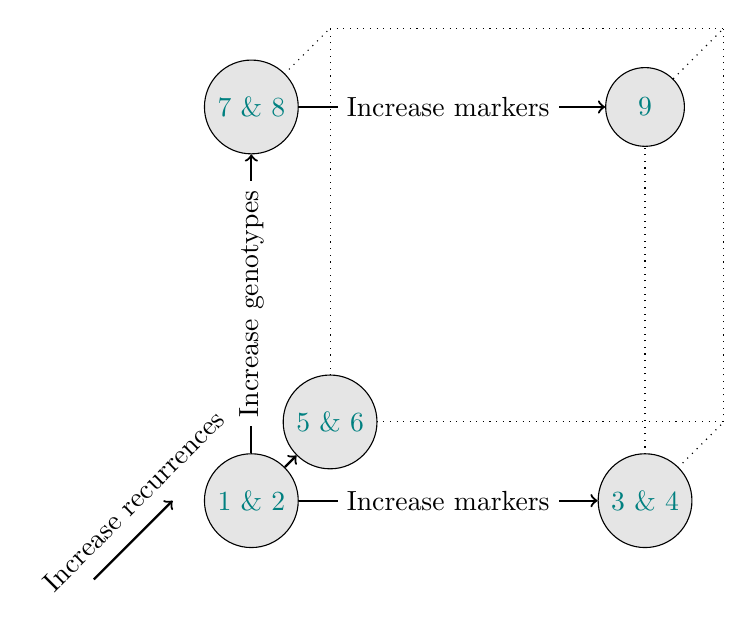
\begin{tikzpicture}

    \tikzstyle{geno} = [draw, circle, rounded corners, minimum height=1cm, minimum width=1cm, fill=gray!20, text=teal]

    % Non-arrow lines
    \draw[dotted,-] (5,0) -- (6,1);
    \draw[dotted,-] (1,1) -- (6,1);
    \draw[dotted,-] (0,5) -- (1,6);
    \draw[dotted,-] (1,6) -- (6,6);
    \draw[dotted,-] (6,1) -- (6,6);
    \draw[dotted,-] (1,1) -- (1,6);
    \draw[dotted,-] (5,0) -- (5,5);
    \draw[dotted,-] (5,5) -- (6,6);

    % Nodes
    \node[geno] at (0,0) (1) {1 \& 2};
    \node[geno] at (5,0) (2) {3 \& 4};
    \node[geno] at (1,1) (3) {5 \& 6};
    \node[geno] at (0,5) (4) {7 \& 8};
    \node[geno] at (5,5) (5) {9};

    % Arrows
    \draw[thick,->] (1) -- (2);
    \draw[thick,->] (1) -- (4);
    %\draw[thick,->] (2) -- (6);
    \draw[thick,->] (4) -- (5);
    \draw[thick,->] (1) -- (3);
    %\draw[thick,->] (6) -- (8);
    \draw[thick,->] (-2,-1) -- (-1,0);

    % Labels
    \node[fill = white] at (2.5,0) {Increase markers};
    \node[fill = white] at (2.5,5) {Increase markers};
    \node[fill = white, rotate = 90] at (0,2.5) {Increase genotypes};
    \node[rotate = 45] at (-1.5,0)
    {Increase recurrences};

    \end{tikzpicture}

\end{center}
    \caption{Visual summary of the examples. We start in the simplest setting (examples \ref{ex:simplest_het} \& \ref{ex:simplest_hom}). We then add complexity in three separate directions: by increasing the number of markers (examples \ref{ex:multiple_markers_het} \& \ref{ex:multiple_markers_hom}), by increasing the number of recurrences (example \ref{ex:multiple_recurs_het} \& \ref{ex:multiple_recurs_hom}), and by increasing the number of genotypes per infection (examples \ref{ex:multiple_genos} \& \ref{ex:cells}), where the latter focuses on the computation of the probability of phased alleles given an IBD partition, to better illustrate how cells are multiplied over. Our final example addresses the need to phase, which can occur when there are multiple genotypes per infection and multiple markers typed (example \ref{ex:phase}).}
    \label{fig:my_label}
\end{figure}

\subsection{Single heterologous marker}\label{ex:simplest_het}

\paragraph{Observed and phased alleles} Suppose a single allele is observed at a single marker, indexed by $j$, genotyped in an enrolment infection, $t=0$, and single recurrent infection, $t=1$. Since we detect only one allele per infection we assume there is only one genotype per infection, indexed by $i$, and one way to phase the observed alleles, e.g., 
\begin{equation*}
    \bm{y} = 
    \begin{blockarray}{cl}
    j=1 \\
    \begin{block}{(c)l}
    \{A\} & t=0 \\
    \{T\} & t=1 \\
    \end{block}
    \end{blockarray},
    \hspace{1cm}
    \bm{a} = 
    \begin{blockarray}{cl}
    j=1 \\
    \begin{block}{(c)l}
    A & i=1 \\
    T & i=2. \\
    \end{block}
    \end{blockarray}
\end{equation*}

\paragraph{Relationship graphs}
To compute the posterior probability of the single recurrent state, $s$, being either a relapse, $L$, reinfection, $I$, or recrudescence $C$, we sum over three graphs ($\rg_\RN{1}$, $\rg_\RN{2}, \rg_\RN{3}$) of relationships between parasite genotypes 1 and 2,  
\begin{center}
    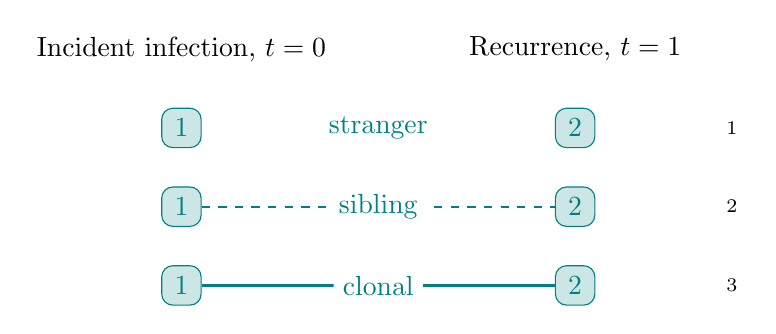
\begin{tikzpicture}

    \tikzstyle{geno} = [draw, rectangle, rounded corners, minimum height=0.5cm, minimum width=0.5cm, color = teal, fill = teal!20]

    % Labels
    \node at (7,0) {$\rg_\RN{1}$};
    \node at (7,-1) {$\rg_\RN{2}$};
    \node at (7,-2) {$\rg_\RN{3}$};
    \node at (0,1) {Incident infection, $t=0$};
    \node at (5,1) {Recurrence, $t=1$};

    % Nodes
    \node[geno] at (0,0) (y1G1) {$1$};
    \node[geno] at (5,0) (y2G1) {$2$};
    \node[geno] at (0,-1) (y1G2) {$1$};
    \node[geno] at (5,-1) (y2G2) {$2$};
    \node[geno] at (0,-2) (y1G3) {$1$};
    \node[geno] at (5,-2) (y2G3) {$2$};

    % Lines
    \path (y1G1) -- (y2G1) node[text = teal, midway]{stranger};
    \draw[geno, dashed, thick] (y1G2) -- (y2G2) node[midway,fill=white]{sibling};
    \draw[geno, thick] (y1G3) -- (y2G3) node[midway,fill=white]{clonal}; 
    \end{tikzpicture}
\end{center}

\paragraph{IBD partitions}
For each relationship graph, we sum over two IBD partitions of genotypes 1 and 2 at the single marker, $\ip_\RN{1} = \{\{1\},\{2\}\}$ and $\ip_\RN{2} = \{\{1,2\}\}$ that correspond to the following two IBD graphs. 
\begin{center}
    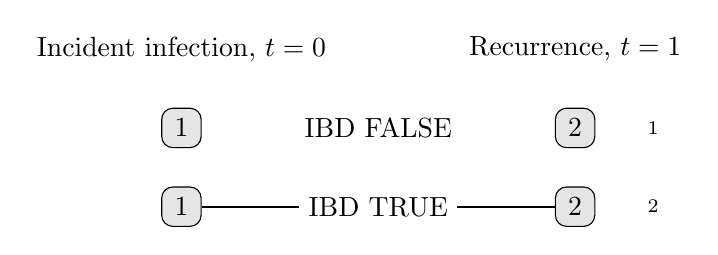
\begin{tikzpicture}

    \tikzstyle{geno} = [draw, rectangle, rounded corners, minimum height=0.5cm, minimum width=0.5cm, fill=gray!20]

    % Labels
    \node at (6,0) {$\ip_\RN{1}$};
    \node at (6,-1) {$\ip_\RN{2}$};
    \node at (0,1) {Incident infection, $t=0$};
    \node at (5,1) {Recurrence, $t=1$};

    % Nodes
    \node[geno] at (0,0) (y1G1) {$1$};
    \node[geno] at (5,0) (y2G1) {$2$};
    \node[geno] at (0,-1) (y1G2) {$1$};
    \node[geno] at (5,-1) (y2G2) {$2$};

    % Lines
    \path (y1G1) -- (y2G1) node[midway]{IBD FALSE};
    \draw[thick] (y1G2) -- (y2G2) node[midway,fill=white]{IBD TRUE};
    
    \end{tikzpicture}
\end{center}

\paragraph{Likelihood} As there is one way to phase the observed alleles and $m=1$, $\mathbb{P}(\bm{y} | s) = \mathbb{P}(\bm{a}|s) = \mathbb{P}(\bm{a}_{\cdot 1}|s)$ where
\small
\begin{equation*}
    \underbrace{
    \begin{blockarray}{lccc}
         & L & I & C \\
        \begin{block}{l(ccc)}
        \bm{a} & \sfrac{1}{2}f(A)f(T) & f(A)f(T) & 0  \\
        \end{block}
        \end{blockarray}
    }_{\mathclap{\mathbb{P}(\bm{a}|s)\forall s\in\{L,I,C\}}}
    =
    \underbrace{
    \begin{blockarray}{ccl}
        \ip_\RN{1} & \ip_\RN{2} \\
        \begin{block}{(cc)l}
          f(A)f(T) & 0 & \bm{a}_{\cdot 1} \\
        \end{block}
        \end{blockarray}
    }_{\mathclap{\mathbb{P}(\bm{a}_{\cdot j}|\ip)\forall\bm{a}_{\cdot j}\in\bm{a}, \ip\in\IP}}
    \times\;
    \underbrace{
    \begin{blockarray}{cccl}
        \rg_\RN{1}, & \rg_\RN{2}, & \rg_\RN{3} & \\
        \begin{block}{(ccc)l}
         1 & \sfrac{1}{2} & 0 & \ip_\RN{1} \\
         0 & \sfrac{1}{2} & 1 & \ip_\RN{2} \\
        \end{block}
        \end{blockarray}
    }_{\mathclap{\mathbb{P}(\ip | \rg)\forall \ip \in \IP, \rg\in\RG}}
    \times\;
    \underbrace{
    \begin{blockarray}{cccc}
        L & I & C & \\
        \begin{block}{(ccc)l}
          \sfrac{1}{3} & 1 & 0 & \rg_\RN{1} \\
          \sfrac{1}{3} & 0 & 0 & \rg_\RN{2} \\
          \sfrac{1}{3} & 0 & 1 & \rg_\RN{3} \\
        \end{block}
        \end{blockarray},
    }_{\mathclap{\mathbb{P}(\rg|s) \forall \rg\in\RG, s\in\{L,I,C\}}}
\end{equation*}
\normalsize
%
and
\begin{align*}
\mathbb{P}(\bm{a}_{\cdot 1} | \ip_\RN{1}) 
&= \mathbb{P}(\{A\} | \{1\}) \times \mathbb{P}(\{T\}|\{2\})
= f(A)f(T).\\
\mathbb{P}(\bm{a}_{\cdot 1} | \ip_\RN{2}) 
&= \mathbb{P}(\{A,T\} | \{1, 2\})
= 0 \text{ because }|\{A,T\}| \neq 1. 
\end{align*}


\paragraph{Posterior} For a uniform prior on $s$, $\mathbb{P}(y) = \sfrac{1}{2}f(A)f(T)$, such that $\mathbb{P}(s = L|\bm{y}) = \sfrac{1}{3}$, $\mathbb{P}(s = I|\bm{y}) = \sfrac{2}{3}$ and $\mathbb{P}(s = C|\bm{y}) = 0$. \\

%=========================================================
\subsection{Single homologous marker} \label{ex:simplest_hom}
For $\bm{y} = (\{A\}, \{A\})^{T}$ and a uniform prior on s, $\mathbb{P}(y) = \sfrac{1}{2}f(A)^2 + \sfrac{1}{2}f(A)$, such that $\mathbb{P}(s = L|\bm{y}) = \sfrac{1}{3}$, $\mathbb{P}(s = I|\bm{y}) = \sfrac{2}{3}f(A)(f(A)+1)^{-1}$ and $\mathbb{P}(s = C|\bm{y}) = \sfrac{2}{3}(f(A)+1)^{-1}$ following
\small
\begin{equation*}
    \underbrace{
    \begin{blockarray}{lccc}
         & L & I & C \\
        \begin{block}{l(ccc)}
        \bm{a} & \sfrac{1}{2}f(A)^2 + \sfrac{1}{2}f(A) & f(A)^2 & f(A)  \\
        \end{block}
        \end{blockarray}
    }_{\mathclap{\mathbb{P}(\bm{a}|s)\forall s\in\{L,I,C\}}}
    =
    \underbrace{
    \begin{blockarray}{ccl}
        \ip_\RN{1} & \ip_\RN{2} \\
        \begin{block}{(cc)l}
          f(A)^2 & f(A) & \bm{a}_{\cdot 1} \\
        \end{block}
        \end{blockarray}
    }_{\mathclap{\mathbb{P}(\bm{a}_{\cdot j}|\ip)\forall \bm{a}_{\cdot j}\in\bm{a}, \ip\in\IP}}
    \times\;
    \underbrace{
    \begin{blockarray}{cccl}
        \rg_\RN{1}, & \rg_\RN{2}, & \rg_\RN{3} & \\
        \begin{block}{(ccc)l}
         1 & \sfrac{1}{2} & 0 & \ip_\RN{1} \\
         0 & \sfrac{1}{2} & 1 & \ip_\RN{2} \\
        \end{block}
        \end{blockarray}
    }_{\mathclap{\mathbb{P}(\ip|\rg)\forall \ip\in\IP, \rg\in\RG}}
    \times\;
    \underbrace{
    \begin{blockarray}{cccc}
        L & I & C & \\
        \begin{block}{(ccc)l}
          \sfrac{1}{3} & 1 & 0 & \rg_\RN{1} \\
          \sfrac{1}{3} & 0 & 0 & \rg_\RN{2} \\
          \sfrac{1}{3} & 0 & 1 & \rg_\RN{3} \\
        \end{block}
        \end{blockarray}.
    }_{\mathclap{\mathbb{P}(\rg|s) \forall \rg\in\RG, s\in\{L,I,C\}}}
\end{equation*}
\normalsize
\subsection{Multiple partially heterologous markers}\label{ex:multiple_markers_het}
% Re-add Allele indices

\paragraph{Observed and phased alleles} In the simplest example a single allele is observed per marker genotyped in an incident and single recurrent infection. Since we detect only one allele per infection we assume there is only one genotype per infection and thus there is only one to phase the observed alleles, e.g., 
\begin{equation*}
    \bm{y} = 
    \begin{blockarray}{cccl}
    j = 1 & j = 2 & j = 3 \\
    \begin{block}{(ccc)l}
    \{A\} & \{T\} & \{G\} & t=0 \\
    \{T\} & \{T\} & \{G\} & t=1 \\
    \end{block}
    \end{blockarray},
    \hspace{1cm}
    \bm{a} = 
    \begin{blockarray}{cccl}
    j = 1 & j = 2 & j = 3\\
    \begin{block}{(ccc)l}
    A & T & G & i=1 \\
    T & T & G & i=2 \\
    \end{block}
    \end{blockarray}.
\end{equation*}


\paragraph{Relationship graphs and IBD partitions} We sum over the same three graphs of relationships between genotypes and the same two IBD partitions as in example \ref{ex:simplest_het}. 

\paragraph{Likelihood} The likelihood computation is similar to examples \ref{ex:simplest_het} \& \ref{ex:simplest_hom}, but because there are multiple markers, which are conditionally independent given the relationship graphs, a product over markers is taken before summing over relationship graphs. In addition, alleles are indexed by $j$, since a given allele at one locus might have a different frequency at another locus. 
\small
\begin{align*}
&\;\mathbb{P}(\bm{y}|s) \forall s\in\{L,I,C\}=
\\
&\; \underbrace{
    \begin{blockarray}{lccc}
        & L & I & C \\
        \begin{block}{l(ccc)}
          \bm{a} & \sfrac{1}{3}f(A_1)f(T_1)f(T_2)f(G_3)\Big(f(T_2)f(G_3) + \sfrac{1}{8}(f(T_2)+1)(f(G_3)+1)\Big)&
          f(A_1)f(T_1)f(T_2)^2f(G_3)^2 & 
          0  \\
        \end{block}
        \end{blockarray}
    }_{\mathclap{\mathbb{P}(\bm{a}|s)\forall s\in\{L,I,C\}}}
    \\
&= \underbrace{
    \begin{blockarray}{lccc}
        & \rg_\RN{1} & \rg_\RN{2} & \rg_\RN{3}\\
        \begin{block}{l(ccc)}
          \bm{a} & f(A_1)f(T_1)f(T_2)^2f(G_3)^2 & 
          \sfrac{1}{8}f(A_1)f(T_1)f(T_2)(f(T_2)+1)f(G_3)(f(G_3)+1)& 
          0  \\
        \end{block}
        \end{blockarray}
    }_{\mathclap{\mathbb{P}(\bm{a}|\rg)\forall\rg\in\RG}}
    \times\;
    \underbrace{
    \begin{blockarray}{cccc}
        L & I & C & \\
        \begin{block}{(ccc)l}
          \sfrac{1}{3} & 1 & 0 & \rg_\RN{1} \\
          \sfrac{1}{3} & 0 & 0 & \rg_\RN{2} \\
          \sfrac{1}{3} & 0 & 1 & \rg_\RN{3} \\
        \end{block}
        \end{blockarray}.
    }_{\mathclap{\mathbb{P}(\rg|s) \forall \rg\in\RG, s\in\{L,I,C\}}}
    \\
&=
\text{row product}
\left\{\;
\underbrace{
    \begin{blockarray}{cccl}
        \rg_\RN{1} & \rg_\RN{2} & \rg_\RN{3}\\
        \begin{block}{(ccc)l}
          f(A_1)f(T_1) & \sfrac{1}{2}f(A_1)f(T_1) & 0 & \bm{a_{\cdot 1}} \\
          f(T_2)^2 & \sfrac{1}{2}f(T_2)^2 + \sfrac{1}{2}f(T_2) & f(T_2) & \bm{a_{\cdot 2}} \\
          f(G_3)^2 & \sfrac{1}{2}f(G_3)^2 + \sfrac{1}{2}f(G_3) & f(G_3) & \bm{a_{\cdot 3}} \\
        \end{block}
        \end{blockarray}
    }_{\mathclap{\mathbb{P}(\bm{a}_{\cdot j}|\rg) \text{ for }j=1,2,3\text{ and all }\rg\in\RG}}
\right\}
    \times\;
    \underbrace{
    \begin{blockarray}{cccc}
        L & I & C & \\
        \begin{block}{(ccc)l}
          \sfrac{1}{3} & 1 & 0 & \rg_\RN{1} \\
          \sfrac{1}{3} & 0 & 0 & \rg_\RN{2} \\
          \sfrac{1}{3} & 0 & 1 & \rg_\RN{3} \\
        \end{block}
        \end{blockarray}.
    }_{\mathclap{\mathbb{P}(\rg|s) \forall \rg\in\RG, s\in\{L,I,C\}}}
    \\
&= 
\text{row product}
    \left\{\;
    \underbrace{
    \begin{blockarray}{ccl}
        \ip_\RN{1} & \ip_\RN{2} \\
        \begin{block}{(cc)l}
          f(A_1)f(T_1) & 0 & \bm{a_{\cdot 1}} \\
          f(T_2)^2 & f(T_2) & \bm{a_{\cdot 2}} \\
          f(G_3)^2 & f(G_3) & \bm{a_{\cdot 3}} \\
        \end{block}
        \end{blockarray}
    }_{\mathclap{\mathbb{P}(\bm{a}_j|\ip) \text{ for }j=1,2,3\text{ and all }\ip\in\IP}}
    \times\;
    \underbrace{
    \begin{blockarray}{cccl}
        \rg_\RN{1}, & \rg_\RN{2}, & \rg_\RN{3} & \\
        \begin{block}{(ccc)l}
         1 & \sfrac{1}{2} & 0 & \ip_\RN{1} \\
         0 & \sfrac{1}{2} & 1 & \ip_\RN{2} \\
        \end{block}
        \end{blockarray}
    }_{\mathclap{\mathbb{P}(\ip | \rg)\forall \ip\in\IP, \rg\in\RG}}
    \right\}
    \times\;
    \underbrace{
    \begin{blockarray}{cccc}
        L & I & C & \\
        \begin{block}{(ccc)l}
          \sfrac{1}{3} & 1 & 0 & \rg_\RN{1} \\
          \sfrac{1}{3} & 0 & 0 & \rg_\RN{2} \\
          \sfrac{1}{3} & 0 & 1 & \rg_\RN{3} \\
        \end{block}
        \end{blockarray}.
    }_{\mathclap{\mathbb{P}(\rg|s) \forall \rg\in\RG, s\in\{L,I,C\}}}
\end{align*}\\
\normalsize

\paragraph{Posterior} For a uniform prior on s, 
\begin{align*}
    \mathbb{P}(\bm{y}) &= \sfrac{1}{3}f(A_1)f(T_1)f(T_2)f(G_3) \Big(\sfrac{1}{3}(f(T_2)f(G_3) + \sfrac{1}{8}(f(T_2)+1)(f(G_3)+1)) + f(T_2)f(G_3) \Big), 
\end{align*}
such that
\begin{align*}
    \mathbb{P}(s=L | \bm{y}) &= 
    \dfrac{\sfrac{1}{3}(f(T_2)f(G_3) + \sfrac{1}{8}(f(T_2)+1)(f(G_3)+1))}
    {\sfrac{1}{3}(f(T_2)f(G_3) + \sfrac{1}{8}(f(T_2)+1)(f(G_3)+1)) + f(T_2)f(G_3)},
    \\
    \mathbb{P}(s=I | \bm{y}) &= 
    \dfrac{f(T_2)f(G_3)}
    {\sfrac{1}{3}(f(T_2)f(G_3) + \sfrac{1}{8}(f(T_2)+1)(f(G_3)+1)) + f(T_2)f(G_3)},
    \\
    \mathbb{P}(s=C | \bm{y}) &= 0.
\end{align*}

%=============================================
\subsection{Multiple exclusively homologous markers}\label{ex:multiple_markers_hom}
When markers are homologous over infections, $\mathbb{P}(s=C | \bm{y}) > 0$. For example, if
\begin{equation*}
\bm{a} = 
    \begin{blockarray}{cccl}
    j = 1 & j = 2 & j = 3\\
    \begin{block}{(ccc)l}
    A & T & G & i=1 \\
    A & T & G & i=2 \\
    \end{block}
    \end{blockarray},    
\end{equation*}
%
\begin{align*}
    \mathbb{P}(\bm{y}) &= 
    \sfrac{1}{9}f(A_1)f(T_2)f(G_3) 
        \Big(\sfrac{1}{8}(f(A_1)+1)(f(T_2)+1)(f(G_3)+1) + 
        4f(A_1)f(T_2)f(G_3) + 4\Big),
\end{align*}
such that
\begin{align*}
    \mathbb{P}(s=L|\bm{y})&= 
    \dfrac{\sfrac{1}{8}(f(A_1)+1)(f(T_2)+1)(f(G_3)+1) 
        + f(A_1)f(T_2)f(G_3) + 1}{
        \sfrac{1}{8}(f(A_1)+1)(f(T_2)+1)(f(G_3)+1) + 
        4f(A_1)f(T_2)f(G_3) + 4},
    \\
    \mathbb{P}(s=I|\bm{y})&= 
    \dfrac{3f(A_1)f(T_2)f(G_3)}
    {\sfrac{1}{8}(f(A_1)+1)(f(T_2)+1)(f(G_3)+1) + 4f(A_1)f(T_2)f(G_3) + 4},
    \\
    \mathbb{P}(s=C|\bm{y})&= 
    \dfrac{3}
    {\sfrac{1}{8}(f(A_1)+1)(f(T_2)+1)(f(G_3)+1) + 4f(A_1)f(T_2)f(G_3) + 4}.\\
\end{align*}

because
\small
\begin{align*}
\mathbb{P}(\bm{y}|s) &= \mathbb{P}(\bm{a}|s) \forall s\in\{L,I,C\}, \\
&= 
\left\{\;
\underbrace{
    \begin{blockarray}{cl}
        \bm{a} \\
        \begin{block}{(c)l}
        \sfrac{1}{3}f(A_1)f(T_2)f(G_3) 
        \Big(f(A_1)f(T_2)f(G_3) +  
        \sfrac{1}{8}(f(A_1)+1)(f(T_2)+1)(f(G_3)+1) 
        + 1\Big)
        & L \\
        f(A_1)^2f(T_2)^2f(G_3)^2 & I \\
        f(A_1)f(T_2)f(G_3) & C \\
        \end{block}
        \end{blockarray},
    }_{\mathclap{\mathbb{P}(\bm{a}|s)\forall s\in\{L,I,C\}}}
\right\}^{T}\\
&= 
\left\{\;
\underbrace{
    \begin{blockarray}{cl}
        \bm{a} \\
        \begin{block}{(c)l}
          f(A_1)^2f(T_2)^2f(G_3)^2 & \rg_\RN{1}\\ 
          \sfrac{1}{8}f(A_1)(f(A_1)+1)f(T_2)(f(T_2)+1)f(G_3)(f(G_3)+1)& \rg_\RN{2} \\
          f(A_1)f(T_2)f(G_3) & \rg_\RN{3} \\
        \end{block}
        \end{blockarray}
    }_{\mathclap{\mathbb{P}(\bm{a}|\rg)\forall\rg\in\RG}}
\right\}^{T}
    \times\;
    \underbrace{
    \begin{blockarray}{cccc}
        L & I & C & \\
        \begin{block}{(ccc)l}
          \sfrac{1}{3} & 1 & 0 & \rg_\RN{1} \\
          \sfrac{1}{3} & 0 & 0 & \rg_\RN{2} \\
          \sfrac{1}{3} & 0 & 1 & \rg_\RN{3} \\
        \end{block}
        \end{blockarray}, 
    }_{\mathclap{\mathbb{P}(\rg|s) \forall \rg\in\RG, s\in\{L,I,C\}}}
    \\
&=
\text{row product}
\left\{\;
\underbrace{
    \begin{blockarray}{cccl}
        \rg_\RN{1} & \rg_\RN{2} & \rg_\RN{3}\\
        \begin{block}{(ccc)l}
          f(A_1)^2 & \sfrac{1}{2}f(A_1)^2 + \sfrac{1}{2}f(A_1) & f(A_1) & \bm{a_{\cdot 1}} \\
          f(T_2)^2 & \sfrac{1}{2}f(T_2)^2 + \sfrac{1}{2}f(T_2) & f(T_2) & \bm{a_{\cdot 2}} \\
          f(G_3)^2 & \sfrac{1}{2}f(G_3)^2 + \sfrac{1}{2}f(G_3) & f(G_3) & \bm{a_{\cdot 3}} \\
        \end{block}
        \end{blockarray}
    }_{\mathclap{\mathbb{P}(\bm{a}_{\cdot j}|\rg) \text{ for }j=1,2,3\text{ and all }\rg\in\RG}}
\right\}
    \times\;
    \underbrace{
    \begin{blockarray}{cccc}
        L & I & C & \\
        \begin{block}{(ccc)l}
          \sfrac{1}{3} & 1 & 0 & \rg_\RN{1} \\
          \sfrac{1}{3} & 0 & 0 & \rg_\RN{2} \\
          \sfrac{1}{3} & 0 & 1 & \rg_\RN{3} \\
        \end{block}
        \end{blockarray},
    }_{\mathclap{\mathbb{P}(\rg|s) \forall \rg\in\RG, s\in\{L,I,C\}}}
    \\
&= 
\text{row product}
    \left\{\;
    \underbrace{
    \begin{blockarray}{ccl}
        \ip_\RN{1} & \ip_\RN{2} \\
        \begin{block}{(cc)l}
          f(A_1)^2 & f(A_1) & \bm{a_{\cdot 1}} \\
          f(T_2)^2 & f(T_2) & \bm{a_{\cdot 2}} \\
          f(G_3)^2 & f(G_3) & \bm{a_{\cdot 3}} \\
        \end{block}
        \end{blockarray}
    }_{\mathclap{\mathbb{P}(\bm{a}_j|\ip) \text{ for }j=1,2,3\text{ and all }\ip\in\IP}}
    \times\;
    \underbrace{
    \begin{blockarray}{cccl}
        \rg_\RN{1}, & \rg_\RN{2}, & \rg_\RN{3} & \\
        \begin{block}{(ccc)l}
         1 & \sfrac{1}{2} & 0 & \ip_\RN{1} \\
         0 & \sfrac{1}{2} & 1 & \ip_\RN{2} \\
        \end{block}
        \end{blockarray}
    }_{\mathclap{\mathbb{P}(\ip | \rg)\forall \ip\in\IP, \rg\in\RG}}
    \right\}
    \times\;
    \underbrace{
    \begin{blockarray}{cccc}
        L & I & C & \\
        \begin{block}{(ccc)l}
          \sfrac{1}{3} & 1 & 0 & \rg_\RN{1} \\
          \sfrac{1}{3} & 0 & 0 & \rg_\RN{2} \\
          \sfrac{1}{3} & 0 & 1 & \rg_\RN{3} \\
        \end{block}
        \end{blockarray}.
    }_{\mathclap{\mathbb{P}(\rg|s) \forall \rg\in\RG, s\in\{L,I,C\}}}
\end{align*}\\
\normalsize
\subsection{More than one recurrence: partially heterologous markers}\label{ex:multiple_recurs_het}

\paragraph{Observed and phased alleles} In the simplest example a single allele is observed at one marker genotyped in an incident infection $t=0$ and in $t=1,2$ recurrent infections. Since we detect only one allele per infection we assume there is only one genotype per infection, s.t. $\bm{y} = \bm{a}$, e.g., 
\begin{align*}
    \bm{y} = 
    \begin{blockarray}{cl}\\
    \begin{block}{(c)l}
    \{A\} & t=0 \\
    \{T\} & t=1 \\
    \{T\} & t=2 \\
    \end{block}
    \end{blockarray},
    \hspace{1cm}
    \bm{a} = 
    \begin{blockarray}{cl}\\
    \begin{block}{(c)l}
    A & i=1 \\
    T & i=2 \\
    T & i=3 \\
    \end{block}
    \end{blockarray}.
\end{align*}

\paragraph{Relationship graphs and IBD partitions}
We sum over 12 relationship graphs, shown below in teal. For each graph, we sum over five IBD partitions $\ip_\RN{1}$ to $\ip_\RN{5}$ which can also be depicted as IBD graphs in grey.  
\begin{align*}
    \ip_\RN{1} &= \{\{1\},\{2\},\{3\}\}, \\
    \ip_\RN{2} &= \{\{1, 2, 3\}\}, \\
    \ip_\RN{3} &= \{\{2, 3\},\{2\}\}, \\
    \ip_\RN{4} &= \{\{1, 2\},\{3\}\}, \\
    \ip_\RN{5} &= \{\{1, 3\},\{2\}\}. \\
\end{align*}
 
\begin{center}
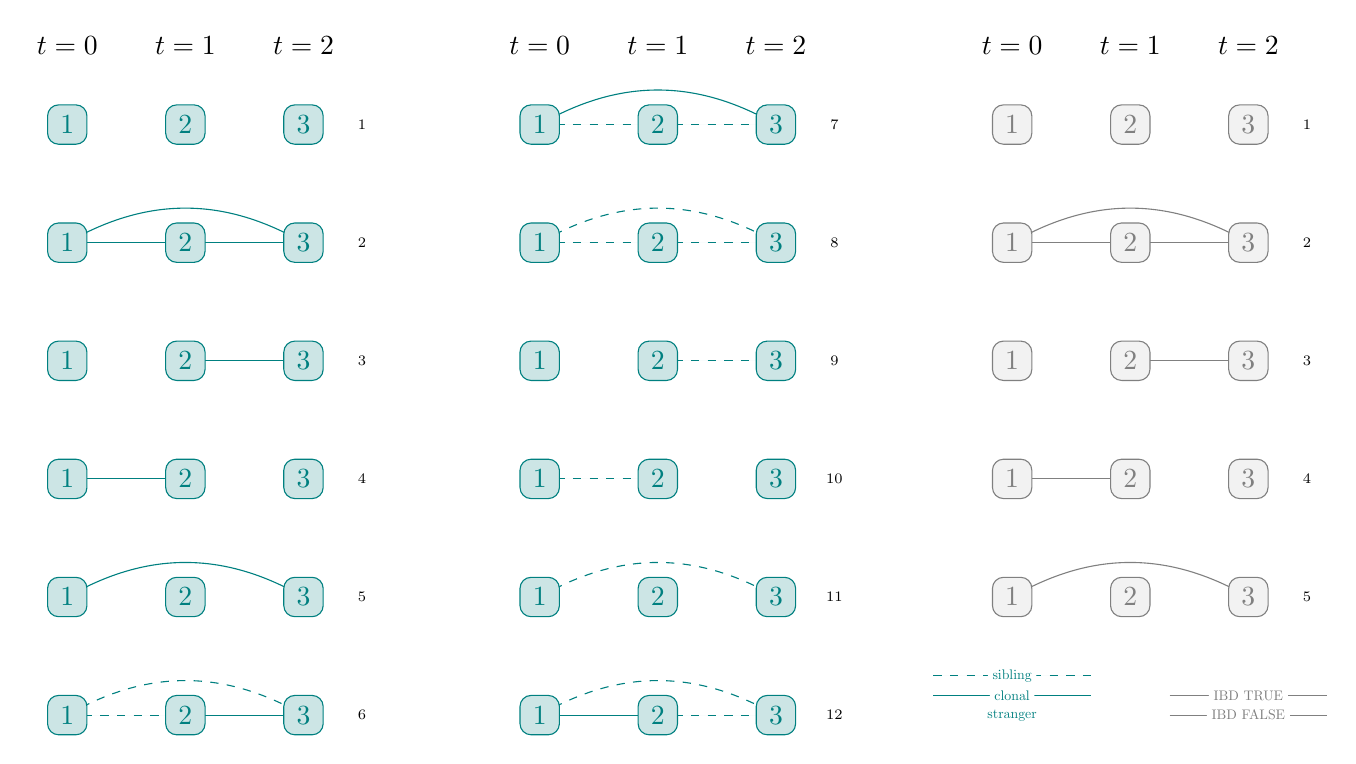
\begin{tikzpicture}
    \tikzstyle{geno} = [draw, rectangle, rounded corners, minimum height=0.5cm, minimum width=0.5cm, color = teal, 
    fill = teal!20]
    
    \tikzstyle{ibd} = [draw, rectangle, rounded corners, minimum height=0.5cm, minimum width=0.5cm, color = gray, 
    fill = gray!10]
    
    \node at (0,1) {$t=0$};
    \node at (1.5,1) {$t=1$};
    \node at (3,1) {$t=2$}; 
    \node at (6,1) {$t=0$};
    \node at (7.5,1) {$t=1$};
    \node at (9,1) {$t=2$}; 
    \node at (12,1) {$t=0$};
    \node at (13.5,1) {$t=1$};
    \node at (15,1) {$t=2$}; 
    \node[scale = 0.75] at (3.75,0) {$\rg_\RN{1}$};
    \node[scale = 0.75] at (3.75,-1.5) {$\rg_\RN{2}$};
    \node[scale = 0.75] at (3.75,-3) {$\rg_\RN{3}$}; 
    \node[scale = 0.75] at (3.75,-4.5) {$\rg_\RN{4}$};
    \node[scale = 0.75] at (3.75,-6) {$\rg_\RN{5}$};
    \node[scale = 0.75] at (3.75,-7.5) {$\rg_\RN{6}$}; 
    \node[scale = 0.75] at (9.75,0) {$\rg_\RN{7}$};
    \node[scale = 0.75] at (9.75,-1.5) {$\rg_\RN{8}$};
    \node[scale = 0.75] at (9.75,-3) {$\rg_\RN{9}$}; 
    \node[scale = 0.75] at (9.75,-4.5) {$\rg_\RN{10}$};
    \node[scale = 0.75] at (9.75,-6) {$\rg_\RN{11}$};
    \node[scale = 0.75] at (9.75,-7.5) {$\rg_\RN{12}$}; 
    \node[scale = 0.75] at (15.75,0) {$\ip_\RN{1}$};
    \node[scale = 0.75] at (15.75,-1.5) {$\ip_\RN{2}$};
    \node[scale = 0.75] at (15.75,-3) {$\ip_\RN{3}$}; 
    \node[scale = 0.75] at (15.75,-4.5) {$\ip_\RN{4}$};
    \node[scale = 0.75] at (15.75,-6) {$\ip_\RN{5}$};
 
    % Graph 1
    \node[geno] at (0,0) {$1$};
    \node[geno] at (1.5,0) {$2$};
    \node[geno] at (3,0) {$3$}; 
    
    % Graph 2
    \path[geno, bend left] (0,-1.5) edge (3,-1.5);
    \draw[geno] (0,-1.5) -- (1.5,-1.5);
    \draw[geno] (1.5,-1.5) -- (3,-1.5);
    \node[geno] at (0,-1.5) {$1$};
    \node[geno] at (1.5,-1.5) {$2$};
    \node[geno] at (3,-1.5) {$3$}; 
    
    % Graph 3
    \draw[geno](1.5,-3) -- (3,-3);
    \node[geno] at (0,-3) {$1$};
    \node[geno] at (1.5,-3) {$2$};
    \node[geno] at (3,-3) {$3$}; 
    
    % Graph 4
    \draw[geno] (0,-4.5) -- (1.5,-4.5);
    \node[geno] at (0,-4.5) {$1$};
    \node[geno] at (1.5,-4.5) {$2$};
    \node[geno] at (3,-4.5) {$3$}; 
    
    % Graph 5
    \path[geno, bend left](0,-6) edge (3,-6);
    \node[geno] at (0,-6) {$1$};
    \node[geno] at (1.5,-6) {$2$};
    \node[geno] at (3,-6) {$3$}; 
    
    % Graph 6
    \path[geno, dashed, bend left] (0,-7.5) edge (3,-7.5);
    \draw[geno, dashed] (0,-7.5) -- (1.5,-7.5);
    \draw[geno] (1.5,-7.5) -- (3,-7.5);
    \node[geno] at (0,-7.5) {$1$};
    \node[geno] at (1.5,-7.5) {$2$};
    \node[geno] at (3,-7.5) {$3$}; 
    
    % Graph 7
    \path[geno, bend left] (6,0) edge (9,0);
    \draw[geno, dashed] (6,0) -- (7.5,0);
    \draw[geno, dashed] (7.5,0) -- (9,0);
    \node[geno] at (6,0) {$1$};
    \node[geno] at (7.5,0) {$2$};
    \node[geno] at (9,0) {$3$}; 
    
    % Graph 8
    \path[geno, dashed, bend left] (6,-1.5) edge (9,-1.5);
    \draw[geno, dashed] (6,-1.5) -- (7.5,-1.5);
    \draw[geno, dashed] (7.5,-1.5) -- (9,-1.5);
    \node[geno] at (6,-1.5) {$1$};
    \node[geno] at (7.5,-1.5) {$2$};
    \node[geno] at (9,-1.5) {$3$}; 
    
    % Graph 9
    \draw[geno, dashed] (7.5,-3) -- (9,-3);
    \node[geno] at (6,-3) {$1$};
    \node[geno] at (7.5,-3) {$2$};
    \node[geno] at (9,-3) {$3$}; 
    
    % Graph 10
    \draw[geno, dashed] (6,-4.5) -- (7.5,-4.5);
    \node[geno] at (6,-4.5) {$1$};
    \node[geno] at (7.5,-4.5) {$2$};
    \node[geno] at (9,-4.5) {$3$}; 
    
    % Graph 11
    \path[geno, dashed, bend left] (6,-6) edge (9,-6);
    \node[geno] at (6,-6) {$1$};
    \node[geno] at (7.5,-6) {$2$};
    \node[geno] at (9,-6) {$3$}; 
    
    % Graph 12
    \path[geno, dashed, bend left] (6,-7.5) edge (9,-7.5);
    \draw[geno] (6,-7.5) -- (7.5,-7.5);
    \draw[geno, dashed] (7.5,-7.5) -- (9,-7.5);
    \node[geno] at (6,-7.5) {$1$};
    \node[geno] at (7.5,-7.5) {$2$};
    \node[geno] at (9,-7.5) {$3$}; 
    
    % Graph 1
    \node[ibd] at (12,0) {$1$};
    \node[ibd] at (13.5,0) {$2$};
    \node[ibd] at (15,0) {$3$}; 
    
    % Graph 2
    \path[ibd, bend left] (12,-1.5) edge (15,-1.5);
    \draw[ibd] (12,-1.5) -- (13.5,-1.5);
    \draw[ibd] (13.5,-1.5) -- (15,-1.5);
    \node[ibd] at (12,-1.5) {$1$};
    \node[ibd] at (13.5,-1.5) {$2$};
    \node[ibd] at (15,-1.5) {$3$}; 
    
    % Graph 3
    \draw[ibd] (13.5,-3) -- (15,-3);
    \node[ibd] at (12,-3) {$1$};
    \node[ibd] at (13.5,-3) {$2$};
    \node[ibd] at (15,-3) {$3$}; 
    
    % Graph 4
    \draw[ibd] (12,-4.5) -- (13.5,-4.5);
    \node[ibd] at (12,-4.5) {$1$};
    \node[ibd] at (13.5,-4.5) {$2$};
    \node[ibd] at (15,-4.5) {$3$}; 
    
    % Graph 5
    \path[ibd, bend left] (12,-6) edge (15,-6);
    \node[ibd] at (12,-6) {$1$};
    \node[ibd] at (13.5,-6) {$2$};
    \node[ibd] at (15,-6) {$3$}; 

    % Legend
    \draw[dashed, geno] (11,-7) -- (13,-7) 
    node[scale=0.5, midway, fill=white]{sibling};
    \draw[geno] (11,-7.25) -- (13,-7.25) 
    node[scale=0.5, midway, fill=white]{clonal};
    \path (11,-7.5) -- (13,-7.5) 
    node[scale=0.5, midway, fill=white, text = teal]{stranger};
    \draw[ibd] (14,-7.25) -- (16,-7.25) 
    node[scale=0.5, midway, fill=white]{IBD TRUE};
    \path[ibd] (14,-7.5) -- (16,-7.5) 
    node[scale=0.5, midway, fill=white]{IBD FALSE};
\end{tikzpicture}
\end{center}


\paragraph{Likelihood} 
Remembering that in linear algebra $(CBA)^T = (A^TB^TC^T)$, 
\small
\begin{align*}
&\mathbb{P}(\bm{y}|\bm{s})\forall\bm{s}\in\{L,I,C\} \times \{L,I,C\} = 
\mathbb{P}(\bm{a}|\bm{s})\forall\bm{s}\in\{L,I,C\} \times \{L,I,C\}, \\
&=\underbrace{ 
    \begin{blockarray}{cl}
    \bm{a} \\
    \begin{block}{(c)l}
    \sfrac{5}{24}f(A)f(T)^2 + \sfrac{9}{48} f(A)f(T) & LL \\
    \sfrac{2}{5}f(A)f(T)^2 + \sfrac{3}{10}f(A)f(T) & IL \\ 
    \sfrac{1}{2}f(A)f(T)^2 & LI \\ 
    \sfrac{1}{2}f(A)f(T) & LC \\ 
    0 & CL \\
    f(A)f(T)^2 & II \\
    0 & CC \\
    f(A)f(T) & IC \\
    0 & CI \\
    \end{block}
    \end{blockarray},
    }_{\mathclap{\mathbb{P}(\bm{a}|\bm{s})\forall\bm{s}\in\{L,I,C\} \times \{L,I,C\}}}
    \\
    &=\underbrace{
    \begin{blockarray}{ccccccccccccl}
        \rg_\RN{1} & \rg_\RN{2} &
        \rg_\RN{3} & \rg_\RN{4} &
        \rg_\RN{5} & \rg_\RN{6} &
        \rg_\RN{7} & \rg_\RN{8} &
        \rg_\RN{9} & \rg_\RN{10} &
        \rg_\RN{11} & \rg_\RN{12} & \\
        \begin{block}{(cccccccccccc)l}
          \sfrac{1}{12} & \sfrac{1}{12} & \sfrac{1}{12} &
          \sfrac{1}{12} & \sfrac{1}{12} & \sfrac{1}{12} &\sfrac{1}{12} & \sfrac{1}{12} & \sfrac{1}{12} &\sfrac{1}{12} & \sfrac{1}{12} & \sfrac{1}{12} 
          & LL \\
          \sfrac{1}{5}&0&\sfrac{1}{5}&
          0&\sfrac{1}{5}&0&0&0&\sfrac{1}{5}&0&\sfrac{1}{5}&0
          & IL \\
          \sfrac{1}{3}&0&0&\sfrac{1}{3}&
          0&0&0&0&0&\sfrac{1}{3}&0&0
          & LI \\
          0&\sfrac{1}{3}&\sfrac{1}{3}&0&
          0&\sfrac{1}{3}&0&0&0&0&0&0
          & LC \\
          0&\sfrac{1}{3}&0&\sfrac{1}{3}&
          0&0&0&0&0&0&0&\sfrac{1}{3}
          & CL \\
          1&0&0&0&0&0&0&0&0&0&0&0& II \\
          0&1&0&0&0&0&0&0&0&0&0&0& CC \\
          0&0&1&0&0&0&0&0&0&0&0&0& IC \\
          0&0&0&1&0&0&0&0&0&0&0&0& CI \\
        \end{block}
        \end{blockarray} 
        }_{_{\mathclap{\mathbb{P}(\rg|\bm{s}) \forall \rg\in\RG, \bm{s}\in\{L,I,C\} \times \{L,I,C\}}}}
    \times 
    \underbrace{
    \begin{blockarray}{cl}
    \bm{a} \\
    \begin{block}{(c)l}
    f(A)f(T)^2 & \rg_\RN{1} \\
    0 & \rg_\RN{2} \\ 
    f(A)f(T) & \rg_\RN{3} \\ 
    0 & \rg_\RN{4} \\ 
    0 & \rg_\RN{5} \\
    \sfrac{1}{2} f(A)f(T) & \rg_\RN{6} \\
    0 & \rg_\RN{7} \\
    \sfrac{1}{4} f(A)f(T) & \rg_\RN{8} \\
    \sfrac{1}{2} f(A)f(T)(f(T) + 1)  & \rg_\RN{9} \\
    \sfrac{1}{2} f(A)f(T)^2 &\rg_\RN{10} \\
    \sfrac{1}{2} f(A)f(T)^2 &\rg_\RN{11} \\
    0 &\rg_\RN{12} \\
    \end{block}
    \end{blockarray}
    }_{\mathclap{\mathbb{P}(\bm{a}|\bm{s})\forall\bm{s}\in\{L,I,C\} \times \{L,I,C\}}}, \\
    &=
    \underbrace{
    \begin{blockarray}{ccccccccccccl}
        \rg_\RN{1} & \rg_\RN{2} &
        \rg_\RN{3} & \rg_\RN{4} &
        \rg_\RN{5} & \rg_\RN{6} &
        \rg_\RN{7} & \rg_\RN{8} &
        \rg_\RN{9} & \rg_\RN{10} &
        \rg_\RN{11} & \rg_\RN{12} & \\
        \begin{block}{(cccccccccccc)l}
          \sfrac{1}{12} & \sfrac{1}{12} & \sfrac{1}{12} &
          \sfrac{1}{12} & \sfrac{1}{12} & \sfrac{1}{12} &\sfrac{1}{12} & \sfrac{1}{12} & \sfrac{1}{12} &\sfrac{1}{12} & \sfrac{1}{12} & \sfrac{1}{12} 
          & LL \\
          \sfrac{1}{5}&0&\sfrac{1}{5}&
          0&\sfrac{1}{5}&0&0&0&\sfrac{1}{5}&0&\sfrac{1}{5}&0
          & IL \\
          \sfrac{1}{3}&0&0&\sfrac{1}{3}&
          0&0&0&0&0&\sfrac{1}{3}&0&0
          & LI \\
          0&\sfrac{1}{3}&\sfrac{1}{3}&0&
          0&\sfrac{1}{3}&0&0&0&0&0&0
          & LC \\
          0&\sfrac{1}{3}&0&\sfrac{1}{3}&
          0&0&0&0&0&0&0&\sfrac{1}{3}
          & CL \\
          1&0&0&0&0&0&0&0&0&0&0&0& II \\
          0&1&0&0&0&0&0&0&0&0&0&0& CC \\
          0&0&1&0&0&0&0&0&0&0&0&0& IC \\
          0&0&0&1&0&0&0&0&0&0&0&0& CI \\
        \end{block}
        \end{blockarray} 
        }_{_{\mathclap{\mathbb{P}(\rg|\bm{s}) \forall \rg\in\RG, \bm{s}\in\{L,I,C\} \times \{L,I,C\}}}}
    \times \quad \\
    &\; \underbrace{ 
    \begin{blockarray}{cccccl}
    \ip_\RN{1} & \ip_\RN{2} & \ip_\RN{3} & 
    \ip_\RN{4} & \ip_\RN{5} \\
    \begin{block}{(ccccc)l}
    1&0&0&0&0&\rg_\RN{1} \\
    0&1&0&0&0&\rg_\RN{2} \\
    0&0&1&0&0&\rg_\RN{3} \\
    0&0&0&1&0&\rg_\RN{4} \\
    0&0&0&0&1&\rg_\RN{5} \\
    0&\sfrac{1}{2}&\sfrac{1}{2}&0&0&\rg_\RN{6} \\
    0&\sfrac{1}{2}&0&0&\sfrac{1}{2}&\rg_\RN{7} \\
    0&\sfrac{1}{4}&\sfrac{1}{4}&\sfrac{1}{4}&\sfrac{1}{4}&\rg_\RN{8} \\
    \sfrac{1}{2}&0&\sfrac{1}{2}&0&0&\rg_\RN{9} \\
    \sfrac{1}{2}&0&0&\sfrac{1}{2}&0&\rg_\RN{10} \\
    \sfrac{1}{2}&0&0&0&\sfrac{1}{2}&\rg_\RN{11} \\
    0&\sfrac{1}{2}&0&\sfrac{1}{2}&0&\rg_\RN{12} \\
    \end{block}
    \end{blockarray}
    }_{\mathclap{\mathbb{P}(\ip|\rg)\forall\ip\in\IP,\rg\in\RG}}
    \times \quad
    \underbrace{ 
    \begin{blockarray}{cl}
    \bm{a}_{\cdot 1} \\
    \begin{block}{(c)l}
    f(A)f(T)^2 & \ip_\RN{1}=\{\{1\},\{2\},\{3\}\} \\
    0 & \ip_\RN{2} = \{\{1, 2, 3\}\} \\ 
    f(A)f(T) & \ip_\RN{3} = \{\{2, 3\},\{2\}\}\\ 
    0 & \ip_\RN{4} = \{\{1, 2\},\{3\}\}\\ 
    0 & \ip_\RN{5} = \{\{1, 3\},\{2\}\}\\
    \end{block}
    \end{blockarray}
    }_{\mathclap{\mathbb{P}(\bm{a}_{\cdot j}|\ip)\forall\bm{a}_{\cdot j}\in\bm{a},\ip\in\IP}}.
\end{align*}


\pagebreak
\paragraph{Posterior}
For a uniform prior on $\bm{s}\in\{L,I,C\}$, 
$\mathbb{P}(\bm{a}) = \tfrac{253}{360}f(A)f(T)^2 + \tfrac{53}{80} f(A)f(T)$ and
\begin{align*}
    \mathbb{P}(s_1 | \bm{y}) \forall s_1\in\{L,I,C\} 
    &=
    {\underbrace{\Big( \tfrac{253}{360}f(A)f(T)^2 + \tfrac{53}{80} f(A)f(T) \Big)
    }_{\mathclap{\mathbb{P}(\bm{y})}}}^{-1} \times \tfrac{1}{3} \times 
    \underbrace{ 
    \begin{blockarray}{cl}
    \begin{block}{(c)l}
    \sfrac{17}{24}f(A)f(T)^2 + \sfrac{11}{16} f(A)f(T) & L \\
    \sfrac{7}{5}f(A)f(T)^2 + \sfrac{13}{10}f(A)f(T) & I \\ 
    0 & C \\
    \end{block}
    \end{blockarray}
    }_{\mathclap{\mathbb{P}(\bm{y}|s_1)\forall s_1\in\{L,I,C\}}}, 
\end{align*}    
    
    
\begin{align*}    
    \mathbb{P}(s_2 | \bm{y}) \forall s_2\in\{L,I,C\} 
    &= 
    {\underbrace{\Big( \tfrac{253}{360}f(A)f(T)^2 + \tfrac{53}{80} f(A)f(T) \Big)
    }_{\mathclap{\mathbb{P}(\bm{y})}}}^{-1} \times \tfrac{1}{3} \times 
    \underbrace{ 
    \begin{blockarray}{cl}
    \begin{block}{(c)l}
    \sfrac{73}{120}f(A)f(T)^2 + \sfrac{39}{80} f(A)f(T) & L \\
    \sfrac{3}{2}f(A)f(T)^2 & I \\ 
    \sfrac{3}{2}f(A)f(T) & C \\
    \end{block}
    \end{blockarray}
    }_{\mathclap{\mathbb{P}(\bm{y}|s_2)\forall s_2\in\{L,I,C\}}}.
\end{align*}

\subsection{More than one recurrence: exclusively homologous markers}\label{ex:multiple_recurs_hom}

If instead $\bm{y} = (\{A\}, \{A\}, \{A\})^{T}$, $\mathbb{P}(\bm{y}|\bm{s}) = \mathbb{P}(\bm{a}|\bm{s})$, which for $\bm{s}=II$ and $\bm{s}=CC$
\begin{align*}
&=\underbrace{ 
    \begin{blockarray}{cl}
    \bm{a} \\
    \begin{block}{(c)l}
    f(A)^3 & II \\
    f(A) & CC \\
    \end{block}
    \end{blockarray},
    }_{\mathclap{\mathbb{P}(\bm{a}|\bm{s})\text{ for } II \text{ and } CC}}
    \\
    &=\underbrace{
    \begin{blockarray}{ccccccccccccl}
        \rg_\RN{1} & \rg_\RN{2} &
        \rg_\RN{3} & \rg_\RN{4} &
        \rg_\RN{5} & \rg_\RN{6} &
        \rg_\RN{7} & \rg_\RN{8} &
        \rg_\RN{9} & \rg_\RN{10} &
        \rg_\RN{11} & \rg_\RN{12} & \\
        \begin{block}{(cccccccccccc)l}
          1&0&0&0&0&0&0&0&0&0&0&0& II \\
          0&1&0&0&0&0&0&0&0&0&0&0& CC \\
        \end{block}
        \end{blockarray} 
        }_{_{\mathclap{\mathbb{P}(\rg|\bm{s}) \text{ for } II \text{ and } CC}}}
    \times 
    \underbrace{
    \begin{blockarray}{cl}
    \bm{a} \\
    \begin{block}{(c)l}
    f(A)^3 & \rg_\RN{1} \\
    f(A) & \rg_\RN{2} \\ 
    f(A)^2 & \rg_\RN{3} \\ 
    f(A)^2 & \rg_\RN{4} \\ 
    f(A)^2 & \rg_\RN{5} \\
    \sfrac{1}{2}(f(A)^2 + f(A)) & \rg_\RN{6} \\
    \sfrac{1}{2}(f(A)^2 + f(A)) & \rg_\RN{7} \\
    \sfrac{1}{4}(3f(A)^2 + f(A)) & \rg_\RN{8} \\
    \sfrac{1}{2}(f(A)^3 + f(A)^2)  & \rg_\RN{9} \\
    \sfrac{1}{2}(f(A)^3 + f(A)^2) &\rg_\RN{10} \\
    \sfrac{1}{2}(f(A)^3 + f(A)^2) &\rg_\RN{11} \\
    \sfrac{1}{2}(f(A)^2 + f(A)) &\rg_\RN{12} \\
    \end{block}
    \end{blockarray}
    }_{\mathclap{\mathbb{P}(\bm{a}|\rg)\forall\rg\in\RG}}, \\
    &= \mathbb{P}(\rg|\bm{s}) \text{ for } II \text{ and } CC \times 
    \underbrace{ 
    \begin{blockarray}{cccccl}
    \ip_\RN{1} & \ip_\RN{2} & \ip_\RN{3} & 
    \ip_\RN{4} & \ip_\RN{5} \\
    \begin{block}{(ccccc)l}
    1&0&0&0&0&\rg_\RN{1} \\
    0&1&0&0&0&\rg_\RN{2} \\
    0&0&1&0&0&\rg_\RN{3} \\
    0&0&0&1&0&\rg_\RN{4} \\
    0&0&0&0&1&\rg_\RN{5} \\
    0&\sfrac{1}{2}&\sfrac{1}{2}&0&0&\rg_\RN{6} \\
    0&\sfrac{1}{2}&0&0&\sfrac{1}{2}&\rg_\RN{7} \\
    0&\sfrac{1}{4}&\sfrac{1}{4}&\sfrac{1}{4}&\sfrac{1}{4}&\rg_\RN{8} \\
    \sfrac{1}{2}&0&\sfrac{1}{2}&0&0&\rg_\RN{9} \\
    \sfrac{1}{2}&0&0&\sfrac{1}{2}&0&\rg_\RN{10} \\
    \sfrac{1}{2}&0&0&0&\sfrac{1}{2}&\rg_\RN{11} \\
    0&\sfrac{1}{2}&0&\sfrac{1}{2}&0&\rg_\RN{12} \\
    \end{block}
    \end{blockarray}
    }_{\mathclap{\mathbb{P}(\ip|\rg)\forall\ip\in\IP,\rg\in\RG}}
    \times \quad
    \underbrace{ 
    \begin{blockarray}{cl}
    \bm{a}_{\cdot 1} \\
    \begin{block}{(c)l}
    f(A)^3 & \ip_\RN{1}=\{\{1\},\{2\},\{3\}\}\\
    f(A) & \ip_\RN{2}=\{\{1, 2, 3\}\} \\ 
    f(A)^2 & \ip_\RN{3}=\{\{2, 3\},\{2\}\} \\ 
    f(A)^2 & \ip_\RN{4}=\{\{1, 2\},\{3\}\} \\ 
    f(A)^2 & \ip_\RN{5}=\{\{1, 3\},\{2\}\} \\
    \end{block}
    \end{blockarray}.
    }_{\mathclap{\mathbb{P}(\bm{a}_{\cdot j}|\ip)\forall\bm{a}_{\cdot j}\in\bm{a},\ip\in\IP}}
\end{align*}

\subsection{Simple example for more than one genotype per infection}\label{ex:multiple_genos}

\paragraph{Observed and phased alleles} In a simple example two and one alleles are observed at a single marker genotyped in an incident and single recurrent infection, respectively. We assume the most parsimonious explanation of the data: the number of genotypes in the first and second infections are two and one, respectively. There is no-longer a one-to-one mapping between genotypes and infections over time. Instead, there are two possible allele assignments: 
\begin{equation*}
    \bm{y} = \begin{blockarray}{cc}\\
    j=1\\
        \begin{block}{(c)c}
        \{A,T\}  & t=0\\
        \{T\} & t=1\\
        \end{block}
        \end{blockarray},
        \hspace{1cm}
    \bm{a}_\RN{1} = \begin{blockarray}{cc}\\
    j=1\\
        \begin{block}{(c)c}
        A & i=1, \; t=0\\
        T & i=2, \; t=0\\
        T & i=3, \; t=1\\
        \end{block}
        \end{blockarray},\hspace{1cm}
    \bm{a}_\RN{2} = \begin{blockarray}{cc}\\
    j=1\\
        \begin{block}{(c)c}
        T & i=1, \; t=0\\
        A & i=2, \; t=0\\
        T & i=3, \; t=1\\
        \end{block}
        \end{blockarray}.
\end{equation*}
Since $\bm{a}_\RN{1}$ and $\bm{a}_\RN{2}$ are equivalent up to a swap between the two genotypes in the first episode, we have $s\in\{L,I,C\}$ that $\mathbb{P}(\bm{y}|s) = 2\mathbb{P}(\bm{a}_\RN{1}|s)$.

\paragraph{Relationship graphs and IBD partitions} There are nine relationship graphs (a subset of those in example \ref{ex:multiple_recurs_het} because clonal relationships within infections are disallowed) to sum over and five IBD partitions (the same as those in example \ref{ex:multiple_recurs_het}), corresponding to the same five IBD graphs as follows.

\begin{center}
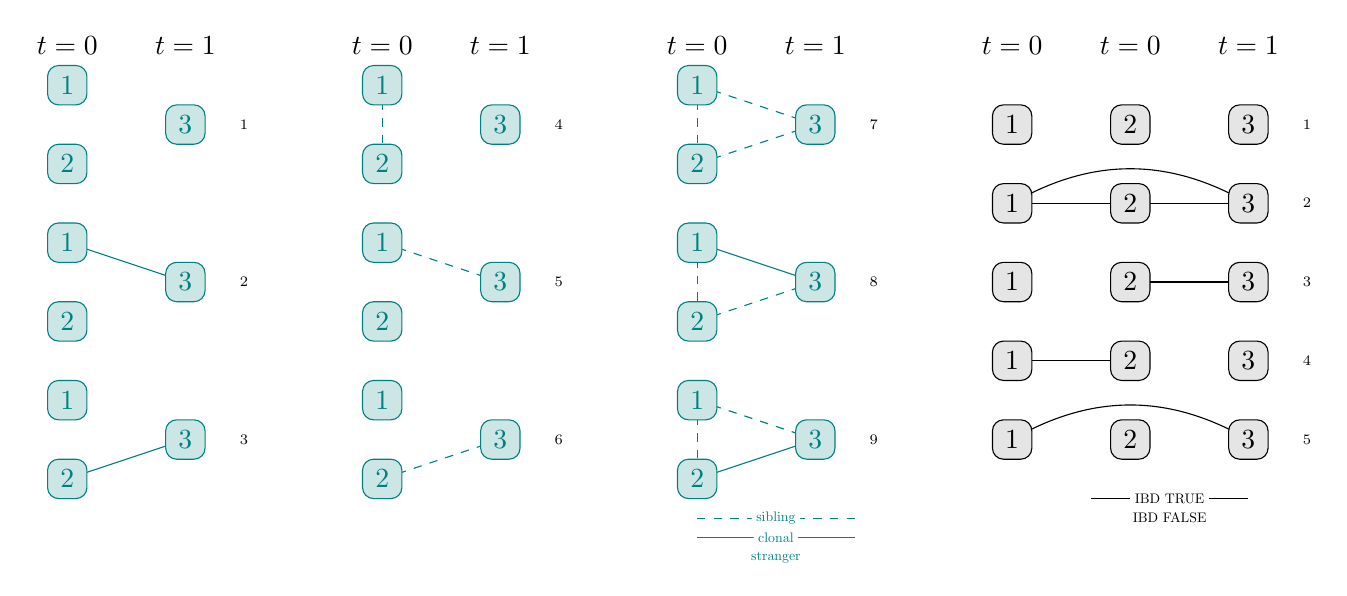
\begin{tikzpicture}
    \tikzstyle{geno} = [draw, rectangle, rounded corners, minimum height=0.5cm, minimum width=0.5cm, color=teal, fill=teal!20]
    \tikzstyle{ibd} = [draw, rectangle, rounded corners, minimum height=0.5cm, minimum width=0.5cm, fill=gray!20]
    
    \node at (0,1) {$t=0$};
    \node at (1.5,1) {$t=1$};
    \node at (4,1) {$t=0$};
    \node at (5.5,1) {$t=1$};
    \node at (8,1) {$t=0$};
    \node at (9.5,1) {$t=1$};
    \node at (12,1) {$t=0$};
    \node at (13.5,1) {$t=0$};
    \node at (15,1) {$t=1$};
    
    \node[scale = 0.75] at (2.25,0) {$\rg_\RN{1}$};
    \node[scale = 0.75] at (2.25,-2) {$\rg_\RN{2}$};
    \node[scale = 0.75] at (2.25,-4) {$\rg_\RN{3}$}; 
    \node[scale = 0.75] at (6.25,0) {$\rg_\RN{4}$};
    \node[scale = 0.75] at (6.25,-2) {$\rg_\RN{5}$};
    \node[scale = 0.75] at (6.25,-4) {$\rg_\RN{6}$}; 
    \node[scale = 0.75] at (10.25,0) {$\rg_\RN{7}$};
    \node[scale = 0.75] at (10.25,-2) {$\rg_\RN{8}$};
    \node[scale = 0.75] at (10.25,-4) {$\rg_\RN{9}$}; 
    \node[scale = 0.75] at (15.75,0) {$\ip_\RN{1}$};
    \node[scale = 0.75] at (15.75,-1) {$\ip_\RN{2}$};
    \node[scale = 0.75] at (15.75,-2) {$\ip_\RN{3}$}; 
    \node[scale = 0.75] at (15.75,-3) {$\ip_\RN{4}$};
    \node[scale = 0.75] at (15.75,-4) {$\ip_\RN{5}$};
 
    % Graph 1
    \node[geno] at (0,0.5) {$1$};
    \node[geno] at (0,-0.5) {$2$};
    \node[geno] at (1.5,0) {$3$}; 
    
    % Graph 2
    \draw[geno](0,-1.5) -- (1.5,-2);
    \node[geno] at (0,-1.5) {$1$};
    \node[geno] at (0,-2.5) {$2$};
    \node[geno] at (1.5,-2) {$3$}; 
    
    % Graph 3
    \draw[geno] (0,-4.5) -- (1.5,-4);
    \node[geno] at (0,-3.5) {$1$};
    \node[geno] at (0,-4.5) {$2$};
    \node[geno] at (1.5,-4) {$3$}; 
    
    % Graph 4
    \draw[geno, dashed](4,0.5) -- (4,-0.5);
    \node[geno] at (4,0.5) {$1$};
    \node[geno] at (4,-0.5) {$2$};
    \node[geno] at (5.5,0) {$3$}; 
    
    % Graph 5
    \draw[geno, dashed](4,-1.5) -- (5.5,-2);
    \node[geno] at (4,-1.5) {$1$};
    \node[geno] at (4,-2.5) {$2$};
    \node[geno] at (5.5,-2) {$3$}; 
    
    % Graph 6
    \draw[geno, dashed](4,-4.5) -- (5.5,-4);
    \node[geno] at (4,-3.5) {$1$};
    \node[geno] at (4,-4.5) {$2$};
    \node[geno] at (5.5,-4) {$3$}; 
    
    % Graph 7
    \draw[geno, dashed](8,0.5) -- (8,-0.5);
    \draw[geno, dashed](9.5,0) -- (8,0.5);
    \draw[geno, dashed](9.5,0) -- (8,-0.5);
    \node[geno] at (8,0.5) {$1$};
    \node[geno] at (8,-0.5) {$2$};
    \node[geno] at (9.5,0) {$3$}; 
    
    % Graph 8
    \draw[geno](8,-1.5) -- (9.5,-2);
    \draw[geno, dashed](9.5,-2) -- (8,-2.5);
    \draw[geno, dashed](8,-1.5) -- (8,-2.5);
    \node[geno] at (8,-1.5) {$1$};
    \node[geno] at (8,-2.5) {$2$};
    \node[geno] at (9.5,-2) {$3$}; 
    
    % Graph 9
    \draw[geno](8,-4.5) -- (9.5,-4);
    \draw[geno, dashed](9.5,-4) -- (8,-3.5);
    \draw[geno, dashed](8,-3.5) -- (8,-4.5);
    \node[geno] at (8,-3.5) {$1$};
    \node[geno] at (8,-4.5) {$2$};
    \node[geno] at (9.5,-4) {$3$}; 
    
    % Graph 1
    \node[ibd] at (12,0) {$1$};
    \node[ibd] at (13.5,0) {$2$};
    \node[ibd] at (15,0) {$3$}; 
    
    % Graph 2
    \path[bend left] (12,-1) edge (15,-1);
    \draw (12,-1) -- (13.5,-1);
    \draw (13.5,-1) -- (15,-1);
    \node[ibd] at (12,-1) {$1$};
    \node[ibd] at (13.5,-1) {$2$};
    \node[ibd] at (15,-1) {$3$}; 
    
    % Graph 3
    \draw (13.5,-2) -- (15,-2);
    \node[ibd] at (12,-2) {$1$};
    \node[ibd] at (13.5,-2) {$2$};
    \node[ibd] at (15,-2) {$3$}; 
    
    % Graph 4
    \draw (12,-3) -- (13.5,-3);
    \node[ibd] at (12,-3) {$1$};
    \node[ibd] at (13.5,-3) {$2$};
    \node[ibd] at (15,-3) {$3$}; 
    
    % Graph 5
    \path[bend left] (12,-4) edge (15,-4);
    \node[ibd] at (12,-4) {$1$};
    \node[ibd] at (13.5,-4) {$2$};
    \node[ibd] at (15,-4) {$3$}; 
    
    % Legend
    \draw[dashed, geno] (8,-5) -- (10,-5) 
    node[scale=0.5, midway, fill=white]{sibling};
    \draw[geno] (8,-5.25) -- (10,-5.25) 
    node[scale=0.5, midway, fill=white]{clonal};
    \path (8,-5.5) -- (10,-5.5) 
    node[scale=0.5, midway, fill=white, text = teal]{stranger};
    \draw (13,-4.75) -- (15,-4.75) 
    node[scale=0.5, midway, fill=white]{IBD TRUE};
    \path (13,-5) -- (15,-5) 
    node[scale=0.5, midway, fill=white]{IBD FALSE};
\end{tikzpicture}
\end{center}

\paragraph{Likelihood} Remembering that in linear algebra $(CBA)^T = (A^TB^TC^T)$, 
\begin{align*}
&\mathbb{P}(\bm{y}|s)\forall s\in\{L,I,C\} = 
2 \underbrace{ 
    \begin{blockarray}{cl}
    \bm{a}_\RN{1} \\
    \begin{block}{(c)l}
    \sfrac{5}{18}f(A)f(T)^2 + \sfrac{1}{4}f(A)f(T) & L \\
    \sfrac{3}{4}f(A)f(T)^2 & I \\ 
    \sfrac{3}{8} f(A)f(T) & C \\ 
    \end{block}
    \end{blockarray}
    }_{\mathclap{\mathbb{P}(\bm{a}_\RN{1}|\bm{s})\forall\bm{s}\in\{L,I,C\}}},
    \\
&=2 \underbrace{
    \begin{blockarray}{cccccccccl}
        \rg_\RN{1} & \rg_\RN{2} & \rg_\RN{3} & 
        \rg_\RN{4} & \rg_\RN{5} & \rg_\RN{6} &
        \rg_\RN{7} & \rg_\RN{8} & \rg_\RN{9}\\
        \begin{block}{(ccccccccc)l}
          \sfrac{1}{9} & \sfrac{1}{9} & \sfrac{1}{9} & 
          \sfrac{1}{9} & \sfrac{1}{9} & \sfrac{1}{9} &
          \sfrac{1}{9} & \sfrac{1}{9} & \sfrac{1}{9} 
          & L \\
          \sfrac{1}{2} &0&0 & \sfrac{1}{2} &0&0&0&0&0 
          & I \\
          0&\sfrac{1}{4}&\sfrac{1}{4}&0&0&0&0&
          \sfrac{1}{4}&\sfrac{1}{4}
          & C \\
        \end{block}
        \end{blockarray}
}_{\mathclap{\mathbb{P}(\rg|s)\forall\rg\in\RG,s\in\{L,I,C\}}} 
\times \quad
\underbrace{ 
    \begin{blockarray}{cl}
    {\bm{a}_\RN{1}}_{\cdot 1} \\
    \begin{block}{(c)l}
    f(A)f(T)^2 & \rg_\RN{1} \\
    0 & \rg_\RN{2} \\ 
    f(A)f(T) & \rg_\RN{3} \\ 
    \sfrac{1}{2}f(A)f(T)^2 & \rg_\RN{4} \\ 
    \sfrac{1}{2}f(A)f(T)^2 & \rg_\RN{5} \\
    \sfrac{1}{2}f(A)f(T)(f(T)+1) &\rg_\RN{6} \\
    \sfrac{1}{4}f(A)f(T) & \rg_\RN{7} \\
    0 &\rg_\RN{8}\\
    \sfrac{1}{2}f(A)f(T) &\rg_\RN{9} \\
    \end{block}
    \end{blockarray}
    }_{\mathclap{\mathbb{P}({\bm{a}_\RN{1}}_{\cdot j}|\rg)\forall{\bm{a}_\RN{1}}_{\cdot j}\in\bm{a}_\RN{1},\rg\in\RG}},
\\
&=2 \underbrace{
    \begin{blockarray}{cccccccccl}
        \rg_\RN{1} & \rg_\RN{2} & \rg_\RN{3} & 
        \rg_\RN{4} & \rg_\RN{5} & \rg_\RN{6} &
        \rg_\RN{7} & \rg_\RN{8} & \rg_\RN{9}\\
        \begin{block}{(ccccccccc)l}
          \sfrac{1}{9} & \sfrac{1}{9} & \sfrac{1}{9} & 
          \sfrac{1}{9} & \sfrac{1}{9} & \sfrac{1}{9} &
          \sfrac{1}{9} & \sfrac{1}{9} & \sfrac{1}{9} 
          & L \\
          \sfrac{1}{2} &0&0 & \sfrac{1}{2} &0&0&0&0&0 
          & I \\
          0&\sfrac{1}{4}&\sfrac{1}{4}&0&0&0&0&
          \sfrac{1}{4}&\sfrac{1}{4}
          & C \\
        \end{block}
        \end{blockarray}
}_{\mathclap{\mathbb{P}(\rg|s)\forall\rg\in\RG,s\in\{L,I,C\}}} 
\times \\
&\underbrace{ 
    \begin{blockarray}{cccccl}
    \ip_\RN{1} & \ip_\RN{2} & \ip_\RN{3} & 
    \ip_\RN{4} & \ip_\RN{5} \\
    \begin{block}{(ccccc)l}
    1&0&0&0&0&\rg_\RN{1} \\
    0&0&0&0&1&\rg_\RN{2} \\
    0&0&1&0&0&\rg_\RN{3}  \\
    \sfrac{1}{2}&0&0&\sfrac{1}{2}&0&\rg_\RN{4} \\
    \sfrac{1}{2}&0&0&0&\sfrac{1}{2}&\rg_\RN{5} \\
    \sfrac{1}{2}&0&\sfrac{1}{2}&0&0&\rg_\RN{6} \\
    0&\sfrac{1}{4}&\sfrac{1}{4}&\sfrac{1}{4}&\sfrac{1}{4}&\rg_\RN{7} \\
    0&\sfrac{1}{2}&0&0&\sfrac{1}{2}&\rg_\RN{8} \\
    0&\sfrac{1}{2}&\sfrac{1}{2}&0&0&\rg_\RN{9} \\
    \end{block}
    \end{blockarray}
    }_{\mathclap{\mathbb{P}(\ip|\rg)\forall\ip\in\IP,\rg\in\RG}} 
    \times \quad
    \underbrace{ 
    \begin{blockarray}{cl}
    {\bm{a}_\RN{1}}_{\cdot 1} \\
    \begin{block}{(c)l}
    f(A)f(T)^2 & \ip_\RN{1} \\
    0 & \ip_\RN{2} \\ 
    f(A)f(T) & \ip_\RN{3} \\ 
    0 & \ip_\RN{4} \\ 
    0 & \ip_\RN{5} \\
    \end{block}
    \end{blockarray}
    }_{\mathclap{\mathbb{P}({\bm{a}_\RN{1}}_{\cdot j}|\ip)\forall{\bm{a}_\RN{1}}_{\cdot j}\in\bm{a}_\RN{1},\ip\in\IP}}.
\end{align*}

\noindent
The prefactor of 2 corresponds to $\A$ consisting of an equivalence class of 2 allele assignments. Note that if the data for the incident infection and the recurrence were reversed, e.g. if $\bm{y}_{t=0} = \{T\}$ and $\bm{y}_{t=1} = \{A,T\}$, the posterior probability of recrudescence would be zero because recrudescences must have the same or fewer genotypes than the directly preceding infection. 

\paragraph{Posterior} For a uniform prior on $s\in\{L,I,C\}$, $\mathbb{P}(\bm{y}) = \tfrac{1}{3}\Big(\tfrac{37}{36}f(A)f(T)^2 + \tfrac{5}{8}f(A)f(T)\Big)$ and 
\begin{equation*}
    \mathbb{P}(s_1 | \bm{y}) \forall s_1\in\{L,I,C\} 
    =
    {\underbrace{\Big(\tfrac{37}{108}f(A)f(T)^2 + \tfrac{5}{24}f(A)f(T)\Big)
    }_{\mathclap{\mathbb{P}(\bm{y})}}}^{-1} \times \tfrac{1}{3} \times 
    \underbrace{ 
    \begin{blockarray}{cl}
    \begin{block}{(c)l}
    \sfrac{5}{18}f(A)f(T)^2 + \sfrac{1}{4}f(A)f(T) & L \\
    \sfrac{3}{4}f(A)f(T)^2 & I \\ 
    \sfrac{3}{8} f(A)f(T) & C \\ 
    \end{block}
    \end{blockarray}
    }_{\mathclap{\mathbb{P}(\bm{y}|\bm{s})\forall\bm{s}\in\{L,I,C\}}},
\end{equation*}

\subsection{Simple zoomed-in example for six genotypes}\label{ex:cells}

\paragraph{Observed and phased alleles} Suppose the observed alleles suggest there are $n>3$ genotypes, e.g., 
\begin{align*}
    \bm{y} = 
    \begin{blockarray}{cl}\\
    j=1\\
    \begin{block}{(c)l}
    \{A,T,C\} & t=0 \\
    \{A,T\} & t=1 \\
    \{A\} & t=2 \\
    \end{block}
    \end{blockarray},
    \hspace{1cm}
    \bm{a} = 
    \begin{blockarray}{cl}\\
    j=1 \\
    \begin{block}{(c)l}
    A & i=1 \\
    T & i=2 \\
    C & i=3 \\
    A & i=4 \\
    T & i=5 \\
    A & i=6 \\
    \end{block}
    \end{blockarray}.
\end{align*}

\paragraph{IBD partitions}
For $n=6$, there are 203 IBD partitions in $\IP$. Three examples, depicted below as graphs, are:  
\begin{align*}
    \ip_\RN{1} &= \{\{\{1,4,6\},\{2,5\},\{3\}\}, \\
    \ip_\RN{2} &= \{\{1,2\},\{3,5\},\{4,6\}\}, \\
    \ip_\RN{3} &= \{\{1\},\{2\},\{3\},\{4\},\{5\},\{6\}\}. \\
\end{align*}
 
\begin{center}
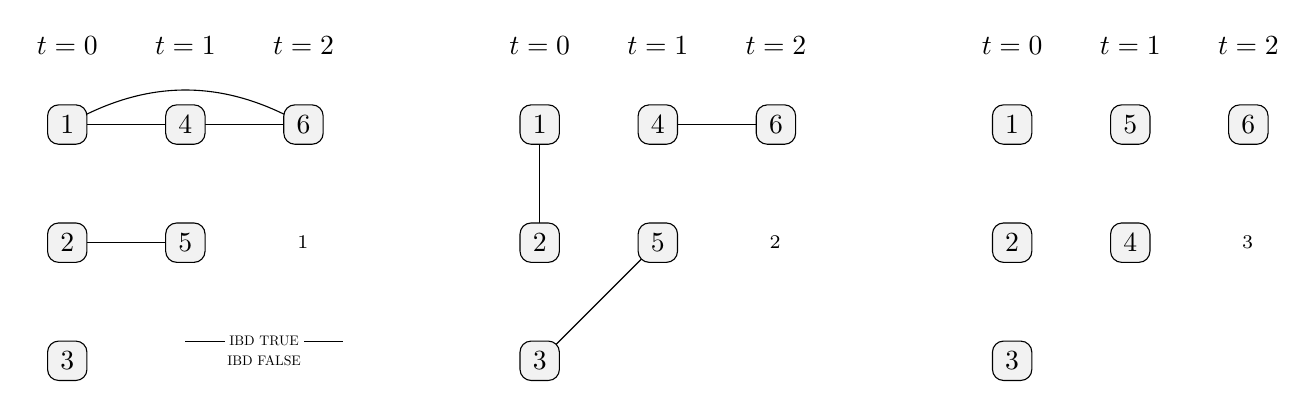
\begin{tikzpicture}
    \tikzstyle{ibd} = [draw, rectangle, rounded corners, minimum height=0.5cm, minimum width=0.5cm, fill = gray!10]
    
    \node at (0,1) {$t=0$};
    \node at (1.5,1) {$t=1$};
    \node at (3,1) {$t=2$}; 
    \node at (6,1) {$t=0$};
    \node at (7.5,1) {$t=1$};
    \node at (9,1) {$t=2$}; 
    \node at (12,1) {$t=0$};
    \node at (13.5,1) {$t=1$};
    \node at (15,1) {$t=2$}; 
   
    % IBD partition
    \path[ibd, bend left] (0,0) edge (3,0);
    \draw[ibd] (0,0) -- (1.5,0);
    \draw[ibd] (1.5,0) -- (3,0);
    \draw[ibd] (0,-1.5) -- (1.5,-1.5);
    \node[ibd] at (0,0) {$1$};
    \node[ibd] at (0,-1.5) {$2$};
    \node[ibd] at (0,-3) {$3$};
    \node[ibd] at (1.5,0) {$4$};
    \node[ibd] at (1.5,-1.5) {$5$};
    \node[ibd] at (3,0) {$6$};
    \node at (3,-1.5) {$\ip_\RN{1}$}; 
    
    % IBD partition
    \draw[ibd] (6,0) -- (6,-1.5);
    \draw[ibd] (6,-3) -- (7.5,-1.5);
    \draw[ibd] (7.5,0) -- (9,0);
    \node[ibd] at (6,0) {$1$};
    \node[ibd] at (6,-1.5) {$2$};
    \node[ibd] at (6,-3) {$3$};
    \node[ibd] at (7.5,0) {$4$};
    \node[ibd] at (7.5,-1.5) {$5$};
    \node[ibd] at (9,0) {$6$}; 
    \node at (9,-1.5) {$\ip_\RN{2}$}; 
    
    % IBD partition
    \node[ibd] at (12,0) {$1$};
    \node[ibd] at (12,-1.5) {$2$};
    \node[ibd] at (12,-3) {$3$};
    \node[ibd] at (13.5,-1.5) {$4$};
    \node[ibd] at (13.5,0) {$5$};
    \node[ibd] at (15,0) {$6$}; 
    \node at (15,-1.5) {$\ip_\RN{3}$}; 

    % Legend
    \draw (1.5,-2.75) -- (3.5,-2.75) 
    node[scale=0.5, midway, fill=white]{IBD TRUE};
    \path (1.5,-3) -- (3.5,-3) 
    node[scale=0.5, midway, fill=white]{IBD FALSE};
\end{tikzpicture}
\end{center}

\begin{align*}
    \mathbb{P}({\bm{a}}_{\cdot 1} | \ip_\RN{1}) 
    &= 
    \mathbb{P}({\bm{a}}_{\{1,4,6\} 1} | \{1,4,6 \}) \times
    \mathbb{P}({\bm{a}}_{\{2,5\} 1} | \{2,5 \}) \times
    \mathbb{P}(a_{3 1} | \{3\}), \\
    &= f(A_1) \times f(T_1) \times f(C_1)
    .\\
    % =====
    \mathbb{P}({\bm{a}}_{\cdot 1} | \ip_\RN{2}) 
    &= 
    \mathbb{P}({\bm{a}}_{\{12\} 1} | \{1,2 \}) \times
    \mathbb{P}({\bm{a}}_{\{3,5\} 1} | \{3,5 \}) \times
    \mathbb{P}({\bm{a}}_{\{4,6\} 1} | \{4,6\}), \\
    &= 0 \times 0 \times f(A_1)
    .\\
    \mathbb{P}({\bm{a}}_{\cdot 1} | \ip_\RN{3}) 
    &= 
    \mathbb{P}(a_{11} | \{1\}) \times
    \mathbb{P}(a_{21} | \{2\}) \times
    \mathbb{P}(a_{31} | \{3\}) \times
    \mathbb{P}(a_{41} | \{4\}) \times
    \mathbb{P}(a_{51} | \{5\}) \times
    \mathbb{P}(a_{61} | \{6\}), \\
    &= f(A)^3 \times f(T)^2 \times f(C).
\end{align*} 
\subsection{Simple example involving phasing} \label{ex:phase}

\paragraph{Observed and phased alleles} In a simple example two alleles are observed at two of three markers genotyped in an incident infection, while one allele is observed per marker genotyped in a single recurrent infection. As in example \ref{ex:multiple_genos}, we assume the most parsimonious explanation of the data: the number of genotypes in the first and second infections are two and one, respectively. However, there are now two non-equivalent ways to phase allelic data into $n = 3$ genotypes, 
\begin{align*}
    \bm{y} &= \begin{blockarray}{cccc}
        j=1 & j=2 & j=3  \\
        \begin{block}{(ccc)c}
        \{A,T\} & \{T\} & \{C,G\} & t=0\\
        \{T\} & \{T\} & \{C\} &t=1\\
        \end{block}
        \end{blockarray}, \\
    \bm{a}_\RN{1}  &= \begin{blockarray}{cccc}
        j=1 & j=2 & j=3  \\
        \begin{block}{(ccc)c}
        A & T & C & j=1, \; t=0\\
        T & T & G & j=2, \; t=0\\
        T & T & C & j=3, \; t=1\\
        \end{block}
        \end{blockarray}, 
        \hspace{1cm}    
    \bm{a}_\RN{2} = \begin{blockarray}{cccc}
        j=1 & j=2 & j=3  \\
        \begin{block}{(ccc)c}
        A & T & G & j=1, \; t=0\\
        T & T & C & j=2, \; t=0\\
        T & T & C & j=3, \; t=1\\
        \end{block}
        \end{blockarray}.
\end{align*}
The total number of allele assignments is in fact $\lvert \A \rvert = 4$, which can be partitioned into two equivalence classes of two allele assignments each; $\bm{a}_\RN{1}$ and $\bm{a}_\RN{2}$ are representatives of the two equivalence classes.

\paragraph{Relationship graphs and IBD partitions} We sum over relationship graphs and IBD partitions in example \ref{ex:multiple_genos}. 

\paragraph{Likelihood}
%
\begin{align*}
\mathbb{P}(\bm{y}|\bm{s} = L) &= 
2c \times 
    \tfrac{1}{9}\Big(
    2f(T_1)f(T_2)^2f(C_3) + \\
    &\qquad \qquad \tfrac{3}{8}f(T_1)(f(T_2)^2 + f(T_2))f(C_3) + \\
    &\qquad \qquad \tfrac{1}{8}f(T_1)(f(T_2)^2 + f(T_2))(f(C_3) + 1) +  \\
    &\qquad \qquad \tfrac{1}{8}(f(T_1) + 1)(f(T_1)^2 + f(T_1))f(C_3) +  \\
    &\qquad \qquad \tfrac{1}{8}(f(T_1) + 1)(f(T_1)^2 + f(T_1))(f(C_3)+ 1) + \\
    &\qquad \qquad \tfrac{1}{32}(3f(T_2) + 1) + \tfrac{1}{8}(9f(T_2) + 1)
    \Big),\\
    %
    \mathbb{P}(\bm{y}|\bm{s} = I) &=
    2c \times \tfrac{1}{8}f(T_1)f(T_2)f(C_3)\Big(9f(T_2) + 1\Big),\\    
    %
    \mathbb{P}(\bm{y}|\bm{s} = C) &=
    2c \times \tfrac{1}{32}\Big(9f(T_2) + 1\Big),
\end{align*}
\normalsize
where $c = f(A_1)f(T_1)f(T_2)f(C_3)f(G_3)$. Note that the prefactor of $2$ corresponds to the fact that each equivalence class consists of two allele assignments. \\ 

\noindent
The likelihood can be written as a summation over $\bm{a}_\RN{1}$ and $\bm{a}_\RN{2}$:
\begin{equation*}
\mathbb{P}(\bm{y}|s)\forall s\in\{L,I,C\} = 
2 \left( \mathbb{P}(\bm{a}_\RN{1} |s)\forall s\in\{L,I,C\} + 
\mathbb{P}(\bm{a}_\RN{2} |s)\forall s\in\{L,I,C\} \right)
\end{equation*}
where, with differences between $\bm{a}_\RN{1}$ and $\bm{a}_\RN{2}$ highlighted in blue, 
\scriptsize
\begin{align*}
&\mathbb{P}(\bm{a}_\RN{1} |s)\forall s\in\{L,I,C\} = \\
&\underbrace{
    \begin{blockarray}{lccccccccc}
        & \rg_\RN{1} & \rg_\RN{2} & \rg_\RN{3} & 
        \rg_\RN{4} & \rg_\RN{5} & \rg_\RN{6} &
        \rg_\RN{7} & \rg_\RN{8} & \rg_\RN{9}\\
        \begin{block}{l(ccccccccc)}
          L & \sfrac{1}{9} & \sfrac{1}{9} & \sfrac{1}{9} & 
          \sfrac{1}{9} & \sfrac{1}{9} & \sfrac{1}{9} &
          \sfrac{1}{9} & \sfrac{1}{9} & \sfrac{1}{9} \\
          I& \sfrac{1}{2} &0&0 & \sfrac{1}{2} &0&0&0&0&0 
          \\
          C&0&\sfrac{1}{4}&\sfrac{1}{4}&0&0&0&0&
          \sfrac{1}{4}&\sfrac{1}{4}
          \\
        \end{block}
        \end{blockarray}
}_{\mathclap{\mathbb{P}(\rg|s)\forall\rg\in\RG,s\in\{L,I,C\}}} 
\times 
\underbrace{
 c \times 
    \begin{blockarray}{cl}
    \bm{a}_\RN{1} \\
    \begin{block}{(c)l}
    f(T_1)  f(T_2)^2  f(C_3) & \rg_\RN{1}\\
    0 &\rg_\RN{2} \\ 
    0 &\rg_\RN{3} \\ 
    \sfrac{1}{8}  f(T_1)  \big(f(T_2)^2 + f(T_2)\big)  f(C_3) &\rg_\RN{4} \\ 
    \sfrac{1}{8}  f(T_1) \big(f(T_2)^2 + f(T_2)\big)\big(f(C_3) + 1 \big) &\rg_\RN{5} \\
    \sfrac{1}{8}  (f(T_1) + 1)  \big(f(T_2)^2 + f(T_2)\big)  f(C_3) &\rg_\RN{6} \\
    \sfrac{1}{64} \big(3f(T_2) + 1\big) &\rg_\RN{7} \\
    0 &\rg_\RN{8} \\
    0 &\rg_\RN{9} \\
    \end{block}
    \end{blockarray}
}_{\mathclap{\mathbb{P}(\bm{a}|\rg)\forall\rg\in\RG}}, 
\end{align*}
%
\begin{align*}
&\mathbb{P}(\bm{a}_\RN{2} |s)\forall s\in\{L,I,C\} = \\
&\underbrace{
    \begin{blockarray}{cccccccccl}
        \rg_\RN{1}& \rg_\RN{2} & \rg_\RN{3} & 
        \rg_\RN{4} & \rg_\RN{5} & \rg_\RN{6} &
        \rg_\RN{7} & \rg_\RN{8} & \rg_\RN{9}\\
        \begin{block}{(ccccccccc)l}
          \sfrac{1}{9} & \sfrac{1}{9} & \sfrac{1}{9} & 
          \sfrac{1}{9} & \sfrac{1}{9} & \sfrac{1}{9} &
          \sfrac{1}{9} & \sfrac{1}{9} & \sfrac{1}{9} 
          & L \\
          \sfrac{1}{2} &0&0 & \sfrac{1}{2} &0&0&0&0&0 
          & I \\
          0&\sfrac{1}{4}&\sfrac{1}{4}&0&0&0&0&
          \sfrac{1}{4}&\sfrac{1}{4}
          & C \\
        \end{block}
        \end{blockarray}
}_{\mathclap{\mathbb{P}(\rg|s)\forall\rg\in\RG,s\in\{L,I,C\}}} 
\times 
\underbrace{ 
c \times 
    \begin{blockarray}{cl}
    \bm{a}_\RN{2} \\
    \begin{block}{(c)l}
    f(T_1)  f(T_2)^2  f(C_3) & \rg_\RN{1}\\
    0 &\rg_\RN{2} \\ 
    {\color{blue}f(T_2)}  &\rg_\RN{3} \\ 
    \sfrac{1}{8} f(T_1)  \big(f(T_2)^2 + f(T_2)\big) f(C_3) &\rg_\RN{4} \\ 
    {\color{blue}\sfrac{1}{8}f(T_1) \big(f(T_2)^2 + f(T_2)\big)  f(C_3)} &\rg_\RN{5} \\
    {\color{blue}\sfrac{1}{8}(f(T_1) + 1) \big(f(T_2)^2 + f(T_2)\big)\big(f(C_3) + 1 \big)} &\rg_\RN{6} \\
    \sfrac{1}{64}\big(3f(T_2) + 1\big)&\rg_\RN{7} \\
    0 &\rg_\RN{8} \\
    {\color{blue}  \sfrac{1}{8} (f(T_2) + 1)} &\rg_\RN{9} \\
    \end{block}
    \end{blockarray}
}_{\mathclap{\mathbb{P}(\bm{a}|\rg)\forall\rg\in\RG}},
\end{align*}
%
\normalsize
and where
\small
\begin{align*}
&\underbrace{ c \times 
    \begin{blockarray}{cl}
    \bm{a}_\RN{1} \\
    \begin{block}{(c)l}
    f(T_1) f(T_2)^2 f(C_3) & \rg_\RN{1}\\
    0 &\rg_\RN{2} \\ 
    0 &\rg_\RN{3} \\ 
    \sfrac{1}{8} f(T_1) \big(f(T_2)^2 + f(T_2)\big) f(C_3) &\rg_\RN{4} \\ 
    \sfrac{1}{8} f(T_1) \big(f(T_2)^2 + f(T_2)\big) \big(f(C_3) + 1 \big)  &\rg_\RN{5} \\
    \sfrac{1}{8} (f(T_1)+1) \big(f(T_2)^2 + f(T_2)\big) f(C_3) &\rg_\RN{6} \\
    \sfrac{1}{64} \big(3f(T_2) + 1\big) &\rg_\RN{7} \\
    0 &\rg_\RN{8} \\
    0 &\rg_\RN{9} \\
    \end{block}
    \end{blockarray}
}_{\mathclap{\mathbb{P}(\bm{a}_\RN{1}|\rg)\forall\rg\in\RG}} = 
\underbrace{ 
    \begin{blockarray}{cl}
    \bm{a}_\RN{1} \\
    \begin{block}{(c)l}
    f(A_1)f(T_1)^2 f(T_2)^3  f(C_3)^2f(G_3) & \rg_\RN{1}\\
    0 &\rg_\RN{2} \\ 
    0 &\rg_\RN{3} \\ 
    \sfrac{1}{8} f(A_1)f(T_1)^2 \big(f(T_2)^3 + f(T_2)^2\big) f(C_3)^2f(G_3) &\rg_\RN{4} \\ 
    \sfrac{1}{8} f(A_1)f(T_1)^2 \big(f(T_2)^3 + f(T_2)^2\big) f(C_3)f(G_3)\big(f(C_3) + 1 \big)  &\rg_\RN{5} \\
    %
    \sfrac{1}{8} f(A_1)f(T_1)(f(T_1)+1) \big(f(T_2)^3 + f(T_2)^2\big) f(C_3)^2f(G_3) &\rg_\RN{6} \\
    %
    \sfrac{1}{64} f(A_1)f(T_1) f(T_2)\big(3f(T_2) + 1\big) f(C_3)f(G_3) &\rg_\RN{7} \\
    0 &\rg_\RN{8} \\
    0 &\rg_\RN{9} \\
    \end{block}
    \end{blockarray}
}_{\mathclap{\mathbb{P}(\bm{a}_\RN{1}|\rg)\forall\rg\in\RG}} \\
&= \text{column product}\left\{
\underbrace{ 
    \begin{blockarray}{cccl}
    {\bm{a}_\RN{1}}_{\cdot 1} & {\bm{a}_\RN{1}}_{\cdot 2} & {\bm{a}_\RN{1}}_{\cdot 3} \\
    \begin{block}{(ccc)l}
    f(A_1)f(T_1)^2 & f(T_2)^3 & f(C_3)^2f(G_3) &\rg_\RN{1}\\
    0 & f(T_2)^2 & f(C_3)f(G_3) &\rg_\RN{2} \\ 
    f(A_1)f(T_1) & f(T_2)^2 & 0 &\rg_\RN{3} \\ 
    \sfrac{1}{2}f(A_1)f(T_1)^2 & \sfrac{1}{2}\big(f(T_2)^3 + f(T_2)^2\big) & \sfrac{1}{2}f(C_3)^2f(G_3) &\rg_\RN{4} \\ 
    \sfrac{1}{2}f(A_1)f(T_1)^2 & \sfrac{1}{2}\big(f(T_2)^3 + f(T_2)^2\big) & \sfrac{1}{2}f(C_3)f(G_3)\big(f(C_3) + 1 \big) &\rg_\RN{5} \\
    %
    \sfrac{1}{2}f(A_1)f(T_1)(f(T_1) + 1) & \sfrac{1}{2}\big(f(T_2)^3 + f(T_2)^2\big) & \sfrac{1}{2}f(C_3)^2f(G_3) &\rg_\RN{6} \\
    %
    \sfrac{1}{4}f(A_1)f(T_1) & \sfrac{1}{4}f(T_2)\big(3f(T_2) + 1\big) & \sfrac{1}{4}f(C_3)f(G_3) 
    & \rg_\RN{7} \\
    0 & \sfrac{1}{2}f(T_2)(f(T_2) + 1) & \sfrac{1}{2}f(C_3)f(G_3) & \rg_\RN{8} \\
    \sfrac{1}{2}f(A_1)f(T_1) & \sfrac{1}{2}f(T_2)(f(T_2) + 1) & 0 &\rg_\RN{9} \\
    \end{block}
    \end{blockarray}
}_{\mathclap{\mathbb{P}({\bm{a}_\RN{1}}_{\cdot j}|\rg)\forall {\bm{a}_\RN{1}}_{\cdot j}\in\bm{a}_\RN{1},\rg\in\RG}}
\right\},
\\
&= \text{column product}\left\{
\underbrace{ 
    \begin{blockarray}{cccccl}
    \ip_\RN{1} & \ip_\RN{2} & \ip_\RN{3} & 
    \ip_\RN{4} & \ip_\RN{5} \\
    \begin{block}{(ccccc)l}
    1&0&0&0&0&\rg_\RN{1}\\
    0&0&0&0&1&\rg_\RN{2} \\
    0&0&1&0&0&\rg_\RN{3}  \\
    \sfrac{1}{2}&0&0&\sfrac{1}{2}&0&\rg_\RN{4} \\
    \sfrac{1}{2}&0&0&0&\sfrac{1}{2}&\rg_\RN{5} \\
    \sfrac{1}{2}&0&\sfrac{1}{2}&0&0&\rg_\RN{6} \\
    0&\sfrac{1}{4}&\sfrac{1}{4}&\sfrac{1}{4}&\sfrac{1}{4}&\rg_\RN{7} \\
    0&\sfrac{1}{2}&0&0&\sfrac{1}{2}&\rg_\RN{8} \\
    0&\sfrac{1}{2}&\sfrac{1}{2}&0&0&\rg_\RN{9} \\
    \end{block}
    \end{blockarray}
}_{\mathclap{\mathbb{P}(\ip|\rg)\forall\ip\in\IP,\rg\in\RG}} 
\times \quad
\underbrace{ 
    \begin{blockarray}{cccl}
    {\bm{a}_\RN{1}}_{\cdot 1} & {\bm{a}_\RN{1}}_{\cdot 2} & {\bm{a}_\RN{1}}_{\cdot 3} \\
    \begin{block}{(ccc)l}
    f(A_1)f(T_1)^2 & f(T_2)^3 & f(C_3)^2f(G_3) & \ip_\RN{1} \\
    0 & f(T_2) & 0 & \ip_\RN{2} \\ 
    f(A_1)f(T_1) & f(T_2)^2 & 0 & \ip_\RN{3} \\ 
    0 & f(T_2)^2 & 0 & \ip_\RN{4} \\ 
    0 & f(T_2)^2 & f(C_3)f(G_3) & \ip_\RN{5} \\
    \end{block}
    \end{blockarray}
}_{\mathclap{\mathbb{P}({\bm{a}_\RN{1}}_{\cdot j}|\ip)\forall {\bm{a}_\RN{1}}_{\cdot j} \in \bm{a}_\RN{1},\ip\in\IP}}
\right\},
\end{align*} 
%
and 
\small
%
\begin{align*}
&\underbrace{ 
c \times 
    \begin{blockarray}{cl}
    \bm{a}_\RN{2} \\
    \begin{block}{(c)l}
    f(T_1)  f(T_2)^2  f(C_3) & \rg_\RN{1}\\
    0 &\rg_\RN{2} \\ 
    {\color{blue}f(T_2)}  &\rg_\RN{3} \\ 
    \sfrac{1}{8} f(T_1)  \big(f(T_2)^2 + f(T_2)\big) f(C_3) &\rg_\RN{4} \\ 
    {\color{blue}\sfrac{1}{8}f(T_1) \big(f(T_2)^2 + f(T_2)\big)  f(C_3)} &\rg_\RN{5} \\
    {\color{blue}\sfrac{1}{8}(f(T_1) + 1) \big(f(T_2)^2 + f(T_2)\big)\big(f(C_3) + 1 \big)} &\rg_\RN{6} \\
    \sfrac{1}{64}\big(3f(T_2) + 1\big)&\rg_\RN{7} \\
    0 &\rg_\RN{8} \\
    {\color{blue}  \sfrac{1}{8} (f(T_2) + 1)} &\rg_\RN{9} \\
    \end{block}
    \end{blockarray}
}_{\mathclap{\mathbb{P}(\bm{a}|\rg)\forall\rg\in\RG}}\\ 
&=\underbrace{ 
    \begin{blockarray}{cl}
    \bm{a}_\RN{2} \\
    \begin{block}{(c)l}
    f(A_1)f(T_1)^2 f(T_2)^3 f(C_3)^2f(G_3) & \rg_\RN{1}\\
    0 &\rg_\RN{2} \\ 
    {\color{blue}f(A_1)f(T_1)f(T_2)^2f(C_3)f(G_3)}  &\rg_\RN{3} \\ 
    \sfrac{1}{8} f(A_1)f(T_1)^2 \big(f(T_2)^3 + f(T_2)^2\big)f(C_3)^2f(G_3) &\rg_\RN{4} \\ 
    {\color{blue}\sfrac{1}{8}f(A_1)f(T_1)^2 \big(f(T_2)^3 + f(T_2)^2\big)f(C_3)^2f(G_3)} &\rg_\RN{5} \\
    {\color{blue}\sfrac{1}{8} f(A_1)f(T_1)(f(T_1)+1) \big(f(T_2)^3 + f(T_2)^2\big)  f(C_3)f(G_3)\big(f(C_3) + 1 \big)} &\rg_\RN{6} \\
    \sfrac{1}{64} (f(A_1)f(T_1)f(T_2)\big(3f(T_2) + 1\big) f(C_3)f(G_3) &\rg_\RN{7} \\
    0 &\rg_\RN{8} \\
    {\color{blue}  \sfrac{1}{8} f(A_1)f(T_1)  f(T_2)(f(T_2) + 1) f(C_3)f(G_3)} &\rg_\RN{9} \\
    \end{block}
    \end{blockarray}
}_{\mathclap{\mathbb{P}(\bm{a}_\RN{2}|\rg)\forall\rg\in\RG}} \\
&= \text{column product}\left\{
\underbrace{ 
    \begin{blockarray}{cccl}
    {\bm{a}_\RN{2}}_{\cdot 1} & {\bm{a}_\RN{2}}_{\cdot 2} & {\bm{a}_\RN{2}}_{\cdot 3} \\
    \begin{block}{(ccc)l}
    f(A_1)f(T_1)^2 & f(T_2)^3 & f(C_3)^2f(G_3) &\rg_\RN{1}\\
    0 & f(T_2)^2 & {\color{blue}0} &\rg_\RN{2} \\ 
    f(A_1)f(T_1) & f(T_2)^2 & {\color{blue}f(C_3)f(G_3)} &\rg_\RN{3} \\ 
    %
    \sfrac{1}{2}f(A_1)f(T_1)^2 & \sfrac{1}{2}\big(f(T_2)^3 + f(T_2)^2\big) & \sfrac{1}{2}f(C_3)^2f(G_3) &\rg_\RN{4} \\ 
    \sfrac{1}{2}f(A_1)f(T_1)^2 & \sfrac{1}{2}\big(f(T_2)^3 + f(T_2)^2\big) & {\color{blue}\sfrac{1}{2}f(C_3)^2f(G_3)} &\rg_\RN{5} \\
    \sfrac{1}{2}f(A_1)f(T_1)(T_1 + 1) & \sfrac{1}{2}\big(f(T_2)^3 + f(T_2)^2\big) & {\color{blue}\sfrac{1}{2}f(C_3)f(G_3)\big(f(C_3) + 1\big)} &\rg_\RN{6} \\
    %
    \sfrac{1}{4}f(A_1)f(T_1) & \sfrac{1}{4}f(T_2)\big(3f(T_2) + 1\big) & \sfrac{1}{4}f(C_3)f(G_3) 
    & \rg_\RN{7} \\
    0 & \sfrac{1}{2}f(T_2)(f(T_2) + 1) & {\color{blue}0} & \rg_\RN{8} \\
    \sfrac{1}{2}f(A_1)f(T_1) & \sfrac{1}{2}f(T_2)(f(T_2) + 1) & 
    {\color{blue}\sfrac{1}{2}f(C_3)f(G_3)} &\rg_\RN{9} \\
    \end{block}
    \end{blockarray}
}_{\mathclap{\mathbb{P}({\bm{a}_\RN{2}}_{\cdot j}|\rg)\forall{\bm{a}_\RN{2}}_{\cdot j}\in\bm{a}_\RN{2},\rg\in\RG}}
\right\},
\\
&= \text{column product}\left\{
\underbrace{ 
    \begin{blockarray}{cccccl}
    \ip_\RN{1} & \ip_\RN{2} & \ip_\RN{3} & 
    \ip_\RN{4} & \ip_\RN{5} \\
    \begin{block}{(ccccc)l}
    1&0&0&0&0&\rg_\RN{1}\\
    0&0&0&0&1&\rg_\RN{2} \\
    0&0&1&0&0&\rg_\RN{3}  \\
    \sfrac{1}{2}&0&0&\sfrac{1}{2}&0&\rg_\RN{4} \\
    \sfrac{1}{2}&0&0&0&\sfrac{1}{2}&\rg_\RN{5} \\
    \sfrac{1}{2}&0&\sfrac{1}{2}&0&0&\rg_\RN{6} \\
    0&\sfrac{1}{4}&\sfrac{1}{4}&\sfrac{1}{4}&\sfrac{1}{4}&\rg_\RN{7} \\
    0&\sfrac{1}{2}&0&0&\sfrac{1}{2}&\rg_\RN{8} \\
    0&\sfrac{1}{2}&\sfrac{1}{2}&0&0&\rg_\RN{9} \\
    \end{block}
    \end{blockarray}
}_{\mathclap{\mathbb{P}(\ip|\rg)\forall\ip\in\IP,\rg\in\RG}} 
\times \quad
\underbrace{ 
    \begin{blockarray}{cccl}
    {\bm{a}_\RN{2}}_{\cdot 1} & {\bm{a}_\RN{2}}_{\cdot 2} & {\bm{a}_\RN{2}}_{\cdot 3} \\
    \begin{block}{(ccc)l}
    f(A_1)f(T_1)^2 & f(T_2)^3 & f(C_3)^2f(G_3) & \ip_\RN{1} \\
    0 & f(T_2) & 0 & \ip_\RN{2} \\ 
    f(A_1)f(T_1) & f(T_2)^2 & {\color{blue}f(C_3)f(G_3)} & \ip_\RN{3} \\ 
    0 & f(T_2)^2 & 0 & \ip_\RN{4} \\ 
    0 & f(T_2)^2 & {\color{blue}0} & \ip_\RN{5} \\
    \end{block}
    \end{blockarray}
}_{\mathclap{\mathbb{P}({\bm{a}_\RN{2}}_{\cdot j}|\ip)\forall{\bm{a}_\RN{2}}_{\cdot j} \in\bm{a}_\RN{2},\ip\in\IP}}
\right\}.
\end{align*}



\end{document}
